% ================================================================
%  CDAC Design Engineer E1 — System Software Specialization
%  DETAILED EXAM NOTES — Easy Explanations + MCQ Focused
%  Compile with pdflatex (run TWICE for TOC)
% ================================================================
\documentclass[11pt,a4paper]{article}

%% ---- PACKAGES ----
\usepackage[a4paper, top=2.2cm, bottom=2.2cm, left=2cm, right=2cm]{geometry}
\usepackage[T1]{fontenc}
\usepackage[utf8]{inputenc}
\usepackage{lmodern}
\usepackage{microtype}
\usepackage{amsmath,amssymb}
\usepackage{xcolor}
\usepackage{listings}
\usepackage{booktabs}
\usepackage{tabularx}
\usepackage{longtable}
\usepackage{array}
\usepackage{multirow}
\usepackage{enumitem}
\usepackage{mdframed}
\usepackage{tcolorbox}
\tcbuselibrary{skins,breakable,listings}
\usepackage{fancyhdr}
\usepackage{titlesec}
\usepackage{hyperref}
\usepackage{tikz}
\usetikzlibrary{shapes.geometric,arrows.meta,positioning,fit,calc,decorations.pathreplacing}
\usepackage{graphicx}
\usepackage{setspace}
\usepackage{parskip}
\usepackage{soul}
\usepackage{fontawesome5}
\usepackage{pifont}

%% ---- COLORS ----
\definecolor{darkblue}{RGB}{13,71,161}
\definecolor{medblue}{RGB}{25,118,210}
\definecolor{lightblue}{RGB}{227,242,253}
\definecolor{orange}{RGB}{230,81,0}
\definecolor{lightorange}{RGB}{255,243,224}
\definecolor{green}{RGB}{27,94,32}
\definecolor{lightgreen}{RGB}{232,245,233}
\definecolor{red}{RGB}{183,28,28}
\definecolor{lightred}{RGB}{255,235,238}
\definecolor{purple}{RGB}{74,20,140}
\definecolor{lightpurple}{RGB}{243,229,245}
\definecolor{teal}{RGB}{0,77,64}
\definecolor{lightteal}{RGB}{224,242,241}
\definecolor{codebg}{RGB}{248,249,250}
\definecolor{codekw}{RGB}{0,0,180}
\definecolor{codecomment}{RGB}{60,128,60}
\definecolor{codestring}{RGB}{180,0,0}
\definecolor{codenumber}{RGB}{128,128,128}
\definecolor{darkgray}{RGB}{55,55,55}
\definecolor{midgray}{RGB}{120,120,120}
\definecolor{yellow}{RGB}{255,193,7}
\definecolor{amber}{RGB}{255,111,0}

%% ---- HYPERREF ----
\hypersetup{
  colorlinks=true, linkcolor=darkblue,
  urlcolor=medblue, pdftitle={CDAC DE-E1 Detailed Notes},
  pdfauthor={Anurag}, bookmarksnumbered=true
}

%% ---- PAGE STYLE ----
\pagestyle{fancy}
\fancyhf{}
\fancyhead[L]{\small\color{darkblue}\textbf{CDAC DE-E1 $\cdot$ System Software}}
\fancyhead[R]{\small\color{darkblue}\thepage}
\fancyfoot[C]{\small\color{midgray}\textit{Detailed Notes for Objective Exam --- 60 Minutes}}
\renewcommand{\headrulewidth}{0.5pt}
\renewcommand{\footrulewidth}{0.3pt}

%% ---- SECTION STYLES ----
\titleformat{\section}
  {\Large\bfseries\color{white}}
  {}
  {0em}
  {\colorbox{darkblue}{\parbox{\dimexpr\linewidth-2\fboxsep\relax}{\strut\thesection\enspace\MakeUppercase{#1}}}}
\titleformat{\subsection}
  {\large\bfseries\color{darkblue}}{\thesubsection\enspace}{0em}{}
\titleformat{\subsubsection}
  {\normalsize\bfseries\color{medblue}}{\thesubsubsection\enspace}{0em}{}
\titleformat{\paragraph}[runin]
  {\normalsize\bfseries\color{teal}}{}{0em}{}[:\enspace]
\titlespacing*{\section}{0pt}{14pt}{6pt}
\titlespacing*{\subsection}{0pt}{10pt}{3pt}
\titlespacing*{\subsubsection}{0pt}{7pt}{2pt}

%% ---- TCOLORBOX STYLES ----
\tcbset{
  mykey/.style={
    breakable, enhanced, arc=3pt,
    colback=lightgreen, colframe=green,
    leftrule=5pt, rightrule=0pt, toprule=0pt, bottomrule=0pt,
    title={\faKey\enspace KEY POINT},
    fonttitle=\bfseries\small\color{green},
    coltitle=green,
    attach boxed title to top left={yshift=-2mm,xshift=6pt},
    boxed title style={colback=green,arc=2pt,boxrule=0pt}
  },
  mytrap/.style={
    breakable, enhanced, arc=3pt,
    colback=lightorange, colframe=orange,
    leftrule=5pt, rightrule=0pt, toprule=0pt, bottomrule=0pt,
    title={\faExclamationTriangle\enspace MCQ TRAP --- READ CAREFULLY},
    fonttitle=\bfseries\small\color=orange,
    coltitle=orange,
    attach boxed title to top left={yshift=-2mm,xshift=6pt},
    boxed title style={colback=orange,arc=2pt,boxrule=0pt}
  },
  myanalogy/.style={
    breakable, enhanced, arc=3pt,
    colback=lightpurple, colframe=purple,
    leftrule=5pt, rightrule=0pt, toprule=0pt, bottomrule=0pt,
    title={\faLightbulb\enspace ANALOGY --- Easy to Remember},
    fonttitle=\bfseries\small\color{purple},
    coltitle=purple,
    attach boxed title to top left={yshift=-2mm,xshift=6pt},
    boxed title style={colback=purple,arc=2pt,boxrule=0pt}
  },
  mydef/.style={
    breakable, enhanced, arc=3pt,
    colback=lightblue, colframe=medblue,
    leftrule=5pt, rightrule=0pt, toprule=0pt, bottomrule=0pt,
    title={\faBookOpen\enspace DEFINITION},
    fonttitle=\bfseries\small\color{medblue},
    coltitle=medblue,
    attach boxed title to top left={yshift=-2mm,xshift=6pt},
    boxed title style={colback=medblue,arc=2pt,boxrule=0pt}
  },
  myexample/.style={
    breakable, enhanced, arc=3pt,
    colback=lightteal, colframe=teal,
    leftrule=5pt, rightrule=0pt, toprule=0pt, bottomrule=0pt,
    title={\faCode\enspace EXAMPLE},
    fonttitle=\bfseries\small\color{teal},
    coltitle=teal,
    attach boxed title to top left={yshift=-2mm,xshift=6pt},
    boxed title style={colback=teal,arc=2pt,boxrule=0pt}
  },
  myimportant/.style={
    breakable, enhanced, arc=3pt,
    colback=lightred, colframe=red,
    leftrule=5pt, rightrule=0pt, toprule=0pt, bottomrule=0pt,
    title={\faStar\enspace IMPORTANT --- Frequently Asked},
    fonttitle=\bfseries\small\color{red},
    coltitle=red,
    attach boxed title to top left={yshift=-2mm,xshift=6pt},
    boxed title style={colback=red,arc=2pt,boxrule=0pt}
  }
}
\newtcolorbox{keypoint}{mykey}
\newtcolorbox{mcqtrap}{mytrap}
\newtcolorbox{analogy}{myanalogy}
\newtcolorbox{mydef}{mydef}
\newtcolorbox{myexample}{myexample}
\newtcolorbox{important}{myimportant}

%% ---- CODE LISTINGS ----
\lstdefinestyle{cstyle}{
  backgroundcolor=\color{codebg},
  basicstyle=\ttfamily\small,
  keywordstyle=\color{codekw}\bfseries,
  commentstyle=\color{codecomment}\itshape,
  stringstyle=\color{codestring},
  numberstyle=\tiny\color{codenumber},
  numbers=left, numbersep=6pt,
  frame=single, framerule=0.4pt,
  rulecolor=\color{midgray!40},
  breaklines=true, tabsize=4,
  showstringspaces=false,
  xleftmargin=10pt, xrightmargin=4pt,
  aboveskip=6pt, belowskip=6pt,
  language=C
}
\lstdefinestyle{bashstyle}{
  backgroundcolor=\color{darkgray},
  basicstyle=\ttfamily\small\color{white},
  keywordstyle=\color{yellow},
  commentstyle=\color{midgray},
  numbers=none,
  frame=none,
  breaklines=true, tabsize=4,
  showstringspaces=false,
  xleftmargin=8pt, aboveskip=4pt, belowskip=4pt
}
\lstset{style=cstyle}

%% ---- HELPERS ----
\newcommand{\code}[1]{\texttt{\small\colorbox{codebg}{\color{codekw}#1}}}
\newcommand{\term}[1]{\textbf{\color{darkblue}#1}}
\newcommand{\highlight}[1]{\colorbox{yellow!50}{\textbf{#1}}}
\newcolumntype{L}[1]{>{\raggedright\arraybackslash}p{#1}}
\newcolumntype{C}[1]{>{\centering\arraybackslash}p{#1}}

%% ================================================================
\begin{document}
%% ================================================================

%% ========== COVER PAGE ==========
\begin{titlepage}
\begin{tikzpicture}[remember picture,overlay]
  \fill[darkblue] (current page.north west) rectangle ([yshift=-7.5cm]current page.north east);
  \fill[amber]    ([yshift=-7.5cm]current page.north west)
                  rectangle ([yshift=-8.1cm]current page.north east);
  \fill[codebg]   ([yshift=-8.1cm]current page.north west)
                  rectangle (current page.south east);
\end{tikzpicture}

\vspace*{0.5cm}
{\color{white}\fontsize{28}{34}\selectfont\bfseries CDAC Design Engineer E1}\\[0.5cm]
{\color{white}\fontsize{18}{22}\selectfont System Software Specialization}\\[0.3cm]
{\color{white!80}\large DETAILED NOTES --- MCQ Objective Exam (60 Minutes)}

\vspace{5cm}

\begin{tcolorbox}[
  enhanced, arc=8pt,
  colback=white, colframe=darkblue, boxrule=2pt,
  width=\linewidth
]
\begin{center}
{\large\bfseries\color{darkblue} Syllabus Coverage}
\end{center}
\begin{enumerate}[leftmargin=1.5cm, itemsep=4pt]
  \item[\textbf{U1.}] \textbf{Computer Architecture \& Low-Level System Design}\\
        \small Memory hierarchy, caches, pipelining, virtual memory, TLB, RISC/CISC, interrupts, DMA
  \item[\textbf{U2.}] \textbf{Compiler Toolchain}\\
        \small Preprocessing, lexing, parsing, semantic analysis, IR, optimizations, linking, loading
  \item[\textbf{U3.}] \textbf{Profiling and Debugging}\\
        \small GDB, Valgrind, Sanitizers (ASan/TSan/UBSan), gprof, perf, static analysis
  \item[\textbf{U4.}] \textbf{Parallel Programming}\\
        \small Processes vs threads, pthreads, mutex, semaphore, deadlock, OpenMP, MPI, Amdahl's Law
  \item[\textbf{U5.}] \textbf{Heterogeneous Computing --- CPU-GPU}\\
        \small GPU architecture, CUDA model, memory types, coalescing, data movement, streams, sync
\end{enumerate}
\end{tcolorbox}

\vfill
\begin{flushright}
  {\large\bfseries\color{darkblue} Anurag}\\
  {\color{midgray} CDAC Exam Preparation $\cdot$ \today}
\end{flushright}
\end{titlepage}

\tableofcontents
\clearpage

%% ================================================================
\section{Computer Architecture \& Low-Level System Design}
%% ================================================================

\subsection{Von Neumann vs Harvard Architecture}

\begin{mydef}
\textbf{Von Neumann Architecture:} A computer design where a single, unified memory holds both program instructions and data, connected to the CPU via a single bus.\\[4pt]
\textbf{Harvard Architecture:} A design with \textit{physically separate} memory and buses for instructions and data.
\end{mydef}

\subsubsection{Von Neumann Architecture --- Deep Dive}

Think of Von Neumann as a single-lane road. Instructions and data share the same road (bus). The CPU can either read an instruction \textit{or} read/write data at any given moment --- not both. This is the famous \term{Von Neumann Bottleneck}.

\textbf{Structure:}
\begin{center}
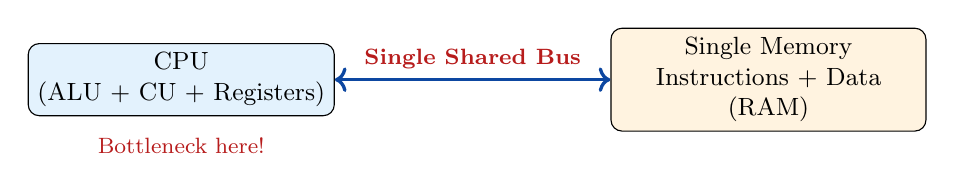
\begin{tikzpicture}[font=\small,
  box/.style={draw,rounded corners,fill=lightblue,minimum width=2.8cm,minimum height=0.9cm,align=center},
  mem/.style={draw,rounded corners,fill=lightorange,minimum width=4cm,minimum height=1.2cm,align=center}
]
  \node[box] (cpu) {CPU\\(ALU + CU + Registers)};
  \node[mem, right=3.5cm of cpu] (mem) {Single Memory\\Instructions + Data\\(RAM)};
  \draw[<->,very thick,darkblue] (cpu) -- node[above,font=\footnotesize\bfseries]{\color{red}Single Shared Bus} (mem);
  \node[below=0.15cm of cpu,font=\footnotesize\color{red}] {Bottleneck here!};
\end{tikzpicture}
\end{center}

\textbf{Key Characteristics:}
\begin{itemize}[noitemsep]
  \item Single address space for code and data
  \item Simple, flexible, general-purpose
  \item Used in: desktops, laptops, servers
  \item The bottleneck: cannot fetch instruction and access data simultaneously
\end{itemize}

\subsubsection{Harvard Architecture --- Deep Dive}

Harvard uses two separate roads (buses). Instructions travel on one road, data on another. The CPU can fetch the next instruction \textit{while simultaneously} reading or writing data. Much faster!

\begin{center}
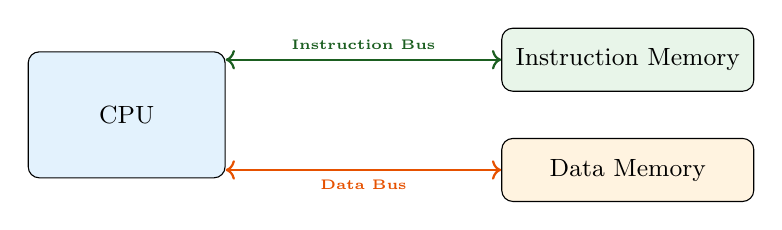
\begin{tikzpicture}[font=\small,
  box/.style={draw,rounded corners,fill=lightblue,minimum width=2.5cm,minimum height=1.6cm,align=center},
  mem/.style={draw,rounded corners,minimum width=3.2cm,minimum height=0.8cm,align=center}
]
  \node[box] (cpu) {CPU};
  \node[mem, right=3.5cm of cpu, yshift=0.7cm, fill=lightgreen] (imem) {Instruction Memory};
  \node[mem, right=3.5cm of cpu, yshift=-0.7cm, fill=lightorange] (dmem) {Data Memory};
  \draw[<->,thick,green] (cpu.east |- imem.west) -- node[above,font=\tiny\bfseries]{Instruction Bus} (imem.west);
  \draw[<->,thick,orange] (cpu.east |- dmem.west) -- node[below,font=\tiny\bfseries]{Data Bus} (dmem.west);
\end{tikzpicture}
\end{center}

\textbf{Key Characteristics:}
\begin{itemize}[noitemsep]
  \item Separate memories and buses for instructions and data
  \item No Von Neumann bottleneck
  \item Used in: microcontrollers (AVR, PIC), DSPs, signal processors
  \item Examples: Arduino (AVR chip internally), ARM Cortex-M series
\end{itemize}

\subsubsection{Modified Harvard Architecture}

Modern CPUs use a clever hybrid:
\begin{itemize}[noitemsep]
  \item \textbf{At the RAM level:} Single unified memory (like Von Neumann)
  \item \textbf{At the cache level:} Separate L1 Instruction Cache and L1 Data Cache (like Harvard)
\end{itemize}

This means the CPU gets the speed of Harvard (separate caches) with the simplicity of Von Neumann (unified RAM).

\textbf{Who uses this?} Intel Core, AMD Ryzen, ARM Cortex-A --- essentially every modern high-performance processor.

\begin{keypoint}
\begin{itemize}[noitemsep]
  \item \textbf{Von Neumann:} Single bus, single memory, general computers
  \item \textbf{Harvard:} Separate buses/memory, microcontrollers/DSPs
  \item \textbf{Modified Harvard:} Unified RAM + split L1 caches, modern CPUs
  \item The Von Neumann bottleneck = CPU can't fetch instruction AND access data simultaneously
\end{itemize}
\end{keypoint}

\begin{mcqtrap}
\begin{itemize}[noitemsep]
  \item Q: ``Which architecture has separate buses for instruction and data?'' $\to$ \highlight{Harvard}
  \item Q: ``Which is used in modern Intel/AMD processors?'' $\to$ \highlight{Modified Harvard}
  \item Q: ``Arduino's AVR chip uses which?'' $\to$ \highlight{Harvard}
  \item Q: ``Which avoids Von Neumann bottleneck?'' $\to$ \highlight{Harvard} (and Modified Harvard)
\end{itemize}
\end{mcqtrap}

%% -------------------------------------------------------------------
\subsection{Memory Hierarchy --- Complete Picture}
%% -------------------------------------------------------------------

\begin{analogy}
Imagine you are a chef (CPU). Your \textbf{hands/pocket} = registers (fastest, tiny). \textbf{Counter beside you} = L1 cache. \textbf{Kitchen shelf} = L2 cache. \textbf{Walk-in pantry} = L3 cache. \textbf{Supermarket} = RAM. \textbf{Warehouse supplier} = SSD/HDD. You always grab from the nearest available location.
\end{analogy}

\begin{center}
\begin{tikzpicture}[font=\small, node distance=0pt]
  \tikzset{
    lvl/.style={draw, trapezium, trapezium left angle=75, trapezium right angle=75,
                fill=#1, minimum width=6cm, minimum height=0.7cm, align=center,
                text width=5.5cm}
  }
  \node[lvl=darkblue!80,text=white] (r)  {Registers $<$1\,ns $\cdot$ Bytes $\cdot$ Compiler managed};
  \node[lvl=darkblue!55,text=white, below=2pt of r]  (l1) {L1 Cache (Split: I\$+D\$) $\cdot$ 1--4\,ns $\cdot$ 32--64\,KB $\cdot$ Per core};
  \node[lvl=darkblue!38, below=2pt of l1] {L2 Cache $\cdot$ 4--12\,ns $\cdot$ 256\,KB--1\,MB $\cdot$ Per core};
  \node[lvl=darkblue!25, below=2pt of l2] (l3) {L3 Cache $\cdot$ 12--40\,ns $\cdot$ 4--32\,MB $\cdot$ Shared across cores};
  \node[lvl=medblue!30, below=2pt of l3] (ram) {RAM (DRAM) $\cdot$ 60--100\,ns $\cdot$ GBs $\cdot$ OS managed};
  \node[lvl=orange!40, below=2pt of ram] (ssd) {SSD/NVMe $\cdot$ 10--100\,\textmu s $\cdot$ TBs};
  \node[lvl=orange!60, below=2pt of ssd] (hdd) {HDD $\cdot$ 5--10\,ms $\cdot$ TBs (slowest)};

  \node[left=0.5cm of r,font=\tiny\bfseries,color=darkblue]  {Fastest};
  \node[left=0.5cm of hdd,font=\tiny\bfseries,color=orange] {Slowest};
  \draw[<->,darkblue,thick] ([xshift=-0.3cm]r.west) -- ([xshift=-0.3cm]hdd.west)
        node[midway,left,font=\tiny,rotate=90,yshift=3pt]{Speed};
\end{tikzpicture}
\end{center}

\textbf{Why multiple levels?} RAM is $\sim$100$\times$ slower than a CPU register. Without caches, CPU would waste most cycles waiting. Caches exploit \term{locality} --- the fact that programs tend to reuse recently or nearby data.

\subsubsection{Locality Principles --- Why Caches Work}

\begin{center}
\begin{tabular}{L{3.5cm} L{5cm} L{5cm}}
\toprule
\textbf{Principle} & \textbf{Meaning} & \textbf{Example} \\
\midrule
\term{Temporal Locality} & If you used data recently, you'll likely use it again soon & Loop counter \code{i} is read thousands of times \\[4pt]
\term{Spatial Locality} & If you accessed address X, you'll likely access addresses near X soon & Array traversal: \code{arr[0]}, \code{arr[1]}, \code{arr[2]}... \\
\bottomrule
\end{tabular}
\end{center}

\subsubsection{Cache Hit and Miss --- The Math}

\begin{itemize}[noitemsep]
  \item \term{Cache Hit:} Data found in cache $\to$ serve at cache speed
  \item \term{Cache Miss:} Data NOT in cache $\to$ fetch from next (slower) level
\end{itemize}

\[
\text{Hit Rate} = \frac{\text{Number of Hits}}{\text{Total Memory Accesses}} \times 100\%
\qquad
\text{Effective Access Time (EAT)} = h \times T_c + (1-h) \times T_m
\]

Where $h$ = hit rate, $T_c$ = cache access time, $T_m$ = main memory access time.

\begin{myexample}
Cache access = 4 ns, RAM access = 100 ns, Hit rate = 95\%.\\
EAT $= 0.95 \times 4 + 0.05 \times 100 = 3.8 + 5 = \mathbf{8.8\ ns}$ (vs 100 ns without cache!)
\end{myexample}

\subsubsection{Types of Cache Misses --- The 3 C's}

\begin{center}
\begin{tabular}{L{3cm} L{5.5cm} L{5.5cm}}
\toprule
\textbf{Miss Type} & \textbf{Cause} & \textbf{Fix} \\
\midrule
\term{Compulsory (Cold)} & First ever access to a block. Cache was empty. Always unavoidable. & Prefetching \\[4pt]
\term{Capacity} & Cache too small to hold the working set. Data was evicted and re-needed. & Increase cache size \\[4pt]
\term{Conflict} & Two blocks map to same cache line and evict each other repeatedly & Increase associativity \\
\bottomrule
\end{tabular}
\end{center}

\subsubsection{Cache Mapping --- How Data is Placed in Cache}

The key question: when you load a block of memory, which cache line does it go into?

\paragraph{Direct Mapped Cache}

Each memory block has \textit{exactly one} possible cache line it can go into. Formula:
\[
\text{Cache Line Index} = \text{Block Address} \bmod N_{\text{cache lines}}
\]

\textbf{Advantage:} Fast to look up (only check one location).\\
\textbf{Disadvantage:} Two frequently used blocks can map to the same line and repeatedly evict each other (\term{thrashing}).

\paragraph{Fully Associative Cache}

A block can go into \textit{any} cache line. When looking for data, the hardware must check \textit{all} lines in parallel.\\
\textbf{Advantage:} Minimum conflict misses.\\
\textbf{Disadvantage:} Expensive hardware, slow for large caches.

\paragraph{N-Way Set Associative Cache (Most Common)}

Compromise: cache is divided into \textit{sets}, each set has N lines. A block maps to one specific set (via mod), but can go in any of the N lines in that set.
\[
\text{Set Index} = \text{Block Address} \bmod N_{\text{sets}}
\]

\textbf{Example:} 4-way set associative $\to$ each set has 4 lines. Modern CPUs typically use 4-way to 16-way.

\begin{center}
\begin{tabular}{C{3.5cm} C{3.5cm} C{3.5cm}}
\toprule
Direct Mapped & N-Way Set Associative & Fully Associative \\
\midrule
1-way sets & N-way sets & One big set \\
Fast lookup & Balanced & Slow lookup \\
High conflict misses & Low conflict misses & Lowest conflict misses \\
\bottomrule
\end{tabular}
\end{center}

\subsubsection{Cache Replacement Policies --- Eviction Strategies}

When a cache is full and a new block must come in, which existing block gets evicted?

\begin{center}
\begin{tabular}{L{3.5cm} L{5.5cm} l}
\toprule
\textbf{Policy} & \textbf{Rule} & \textbf{Used In} \\
\midrule
\term{LRU} (Least Recently Used) & Evict the block not accessed for the longest time. Best performance. & Most CPUs \\[4pt]
\term{FIFO} & Evict the block that was loaded into cache first (oldest). & Simple systems \\[4pt]
\term{LFU} (Least Frequently Used) & Evict the block accessed the fewest times total. & Less common \\[4pt]
\term{Random} & Pick a random block to evict. Simple hardware. & ARM processors \\[4pt]
\term{Clock (Second Chance)} & Circular version of FIFO with a reference bit. LRU approximation. & OS page replacement \\
\bottomrule
\end{tabular}
\end{center}

\subsubsection{Cache Write Policies --- Handling Writes}

When CPU writes data, should we update only cache or also RAM immediately?

\begin{center}
\begin{tabular}{L{3cm} L{5.5cm} L{5.5cm}}
\toprule
& \textbf{Write-Through} & \textbf{Write-Back (Write-Deferred)} \\
\midrule
\textbf{What happens} & Write to both cache AND RAM immediately & Write only to cache; write to RAM when line is evicted \\
\textbf{Speed} & Slower (every write hits RAM) & Faster (writes go to cache only) \\
\textbf{Consistency} & Always consistent & Cache and RAM temporarily differ \\
\textbf{Dirty bit?} & Not needed & \textbf{Yes} --- marks if cache line was modified \\
\textbf{Used when} & Simpler systems & High-performance CPUs \\
\bottomrule
\end{tabular}
\end{center}

\begin{keypoint}
\textbf{Dirty bit} is used in write-back caches. A cache line with dirty bit = 1 means it has been modified and the RAM copy is stale. On eviction, it MUST be written back to RAM.
\end{keypoint}

\subsubsection{MESI Protocol --- Multi-Core Cache Coherence}

\begin{analogy}
Imagine 4 students (CPU cores) each have a personal notebook (L1 cache) and share a single whiteboard (RAM). If student 1 erases something on the whiteboard, how do students 2, 3, 4 know their notebooks are now wrong? MESI solves exactly this.
\end{analogy}

In a multi-core CPU, each core has its own L1/L2 cache. \textbf{Problem:} Core 1 modifies a variable in its cache. Core 2 still has the old value in its cache. They're inconsistent!

\term{MESI Protocol} gives every cache line one of 4 states:

\begin{center}
\begin{tabular}{C{1.5cm} L{4cm} L{4cm} L{4cm}}
\toprule
\textbf{State} & \textbf{Meaning} & \textbf{In this core's cache?} & \textbf{Same as RAM?} \\
\midrule
\textbf{M} Modified  & Only this core has it; modified & Yes (only this core) & \textbf{No} (RAM is stale) \\
\textbf{E} Exclusive & Only this core has it; unmodified & Yes (only this core) & Yes \\
\textbf{S} Shared    & Multiple cores have a copy & Yes & Yes \\
\textbf{I} Invalid   & This copy is stale/unusable & Technically yes but useless & Don't care \\
\bottomrule
\end{tabular}
\end{center}

\textbf{Example Flow:}
\begin{enumerate}[noitemsep]
  \item Core 1 reads \code{x} $\to$ state: \textbf{E} (only in Core 1)
  \item Core 2 reads \code{x} $\to$ both Core 1 and Core 2 get state: \textbf{S} (shared)
  \item Core 1 writes to \code{x} $\to$ Core 1 sends \textbf{Invalidate} broadcast $\to$ Core 2's copy becomes \textbf{I}. Core 1's state $\to$ \textbf{M}
  \item Core 2 tries to read \code{x} $\to$ Cache miss (state was I) $\to$ Core 2 fetches updated value from Core 1 or RAM
\end{enumerate}

\begin{keypoint}
MESI ensures cache coherence in multi-core CPUs. State \textbf{I (Invalid)} means the data MUST be re-fetched. Write to a Shared line $\to$ broadcast Invalidate to all other cores.
\end{keypoint}

%% -------------------------------------------------------------------
\subsection{Pipelining --- Overlapping Instruction Execution}
%% -------------------------------------------------------------------

\begin{mydef}
\textbf{Pipelining:} Breaking instruction execution into multiple stages and overlapping the execution of multiple instructions --- like an assembly line where each stage handles a different instruction simultaneously.
\end{mydef}

\begin{analogy}
Washing clothes: wash $\to$ rinse $\to$ spin $\to$ dry. Without pipelining: finish all 4 steps for load 1, then start load 2. With pipelining: while load 1 is rinsing, load 2 starts washing. All 4 stages run simultaneously on 4 different loads!
\end{analogy}

\subsubsection{Classic 5-Stage RISC Pipeline}

\begin{center}
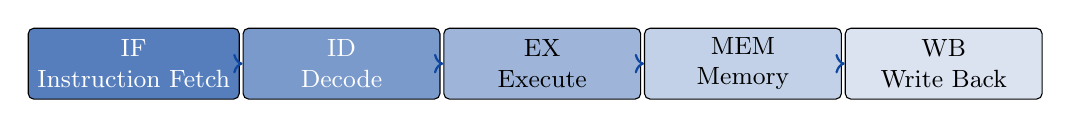
\begin{tikzpicture}[font=\small, node distance=0pt]
  \tikzset{stage/.style={draw,fill=#1,minimum width=2.5cm,minimum height=0.9cm,align=center,rounded corners=2pt}}
  \node[stage=darkblue!70,text=white]  (if) {IF\\Instruction Fetch};
  \node[stage=darkblue!55,text=white, right=1pt of if]  (id) {ID\\Decode};
  \node[stage=darkblue!40, right=1pt of id]  (ex) {EX\\Execute};
  \node[stage=darkblue!25, right=1pt of ex]  (mem) {MEM\\Memory};
  \node[stage=darkblue!15, right=1pt of mem] (wb)  {WB\\Write Back};
  \draw[->,thick,darkblue] (if)--(id); \draw[->,thick,darkblue] (id)--(ex);
  \draw[->,thick,darkblue] (ex)--(mem); \draw[->,thick,darkblue] (mem)--(wb);
\end{tikzpicture}
\end{center}

\begin{center}
\begin{tabular}{C{1.5cm} L{3cm} L{8cm}}
\toprule
\textbf{Stage} & \textbf{Name} & \textbf{What Happens} \\
\midrule
IF  & Instruction Fetch   & Read next instruction from memory (via Program Counter) \\
ID  & Instruction Decode  & Decode the instruction; read source registers from register file \\
EX  & Execute             & ALU performs the operation (arithmetic, logic, address calculation) \\
MEM & Memory Access       & Read or write data from/to RAM (only for load/store instructions) \\
WB  & Write Back          & Write the result to the destination register \\
\bottomrule
\end{tabular}
\end{center}

\textbf{Throughput calculation:}
\begin{itemize}[noitemsep]
  \item Without pipelining: 5 instructions $\times$ 5 cycles = 25 cycles
  \item With pipelining: 5 + (5--1) = 9 cycles to finish 5 instructions
  \item For N instructions: $(5 + N - 1)$ cycles. As $N \to \infty$: throughput $\approx$ 1 instruction/cycle
\end{itemize}

\subsubsection{Pipeline Hazards --- When Pipelining Goes Wrong}

A \term{hazard} is a situation that prevents the pipeline from executing at full speed. There are 3 types:

\paragraph{Type 1: Structural Hazard}

\textbf{Cause:} Two instructions simultaneously need the same physical hardware resource.

\textbf{Classic Example:} Single memory unit. Instruction 1 is in MEM stage (accessing data). Instruction 2 is in IF stage (fetching next instruction). Both need memory at the same time!

\textbf{Solutions:}
\begin{itemize}[noitemsep]
  \item \textbf{Separate I-Cache and D-Cache} (most common) --- this is exactly why Harvard-style split caches exist inside CPUs!
  \item Add duplicate hardware resources
  \item Insert pipeline stalls (bubble/NOP)
\end{itemize}

\paragraph{Type 2: Data Hazard}

\textbf{Cause:} An instruction needs the result of a previous instruction that hasn't finished yet.

\begin{lstlisting}
ADD R1, R2, R3    // Instruction 1: R1 = R2 + R3 (result written in WB stage)
SUB R4, R1, R5    // Instruction 2: needs R1 (in ID stage, but R1 not ready yet!)
\end{lstlisting}

\textbf{3 Types of Data Hazards:}
\begin{center}
\begin{tabular}{L{3.5cm} L{4.5cm} L{6cm}}
\toprule
\textbf{Type} & \textbf{Also Called} & \textbf{Example \& Explanation} \\
\midrule
\term{RAW} Read After Write & \textbf{True Dependency} (most common!) & Instruction 2 reads R1 before Instruction 1 writes R1 \\[4pt]
\term{WAW} Write After Write & Output Dependency & Two instructions write to same register; second write must happen after first \\[4pt]
\term{WAR} Write After Read & Anti-Dependency & Later instruction writes to a register that an earlier instruction still needs to read \\
\bottomrule
\end{tabular}
\end{center}

\textbf{Solutions for Data Hazards:}

\begin{enumerate}[noitemsep]
  \item \term{Forwarding (Bypassing):} Add hardware paths to route the result from EX or MEM output directly back to EX input --- without waiting for WB. Solves most RAW hazards with zero stalls.
  \item \term{Pipeline Stalls (Bubbles):} Insert NOP (no-operation) cycles. Simple but wastes cycles.
  \item \term{Out-of-Order Execution:} Execute instructions whose operands are ready, even if earlier instructions are stalled.
  \item \term{Register Renaming:} Use extra physical registers to create new versions of registers --- eliminates WAW and WAR (which are false dependencies, not true ones).
  \item \term{Compiler Scheduling:} Compiler reorders instructions to place independent instructions between dependent ones.
\end{enumerate}

\paragraph{Type 3: Control Hazard (Branch Hazard)}

\textbf{Cause:} Branch instructions (if/while/for) change the Program Counter. The pipeline has already fetched the next sequential instructions --- which may be wrong!

\begin{lstlisting}
BEQ R1, R2, LABEL   // if R1==R2, jump to LABEL
ADD R3, R4, R5      // Already fetched! But may be wrong if branch taken
SUB R6, R7, R8      // Also already fetched! Might need to discard
\end{lstlisting}

\textbf{Solutions:}

\begin{center}
\begin{tabular}{L{4cm} L{9cm}}
\toprule
\textbf{Solution} & \textbf{How It Works} \\
\midrule
Stall & Pause pipeline until branch resolves. Safe but wastes 1--3 cycles per branch. \\[4pt]
\term{Static Prediction} & Assume branch always NOT taken (or always taken). Simple. Wrong $\sim$30--40\% of time. \\[4pt]
\term{Dynamic Prediction} & Hardware maintains Branch History Table (BHT/BTB). Learns from past outcomes. Modern CPUs: $\sim$95\%+ accuracy. \\[4pt]
\term{Speculative Execution} & Execute along predicted path; discard if wrong. Used in out-of-order CPUs. \\[4pt]
\term{Branch Delay Slot} & Execute one instruction after branch regardless. Compiler fills slot with useful work. Used in MIPS. \\[4pt]
\term{Pipeline Flush} & If prediction was wrong, discard all wrongly-fetched instructions. The penalty = pipeline depth cycles. \\
\bottomrule
\end{tabular}
\end{center}

\begin{important}
\textbf{Branch Misprediction Penalty:} In a deep pipeline (e.g., 15 stages), a mispredicted branch can waste 14 cycles! This is why branch prediction accuracy is so critical in modern CPUs. Spectre/Meltdown vulnerabilities exploited speculative execution.
\end{important}

\begin{keypoint}
\begin{itemize}[noitemsep]
  \item Structural hazard $\to$ duplicate hardware (separate caches)
  \item RAW hazard (most common) $\to$ forwarding/bypassing
  \item WAW/WAR hazard $\to$ register renaming
  \item Control hazard $\to$ branch prediction + speculative execution
\end{itemize}
\end{keypoint}

\begin{mcqtrap}
\begin{itemize}[noitemsep]
  \item ``WAR and WAW are solved by?'' $\to$ \highlight{Register Renaming} (NOT forwarding!)
  \item ``Which hazard is most common?'' $\to$ \highlight{RAW (Read After Write)}
  \item ``Forwarding solves which hazard?'' $\to$ \highlight{RAW (Data hazard)}
  \item ``Branch misprediction causes?'' $\to$ \highlight{Pipeline Flush} (instructions discarded)
\end{itemize}
\end{mcqtrap}

%% -------------------------------------------------------------------
\subsection{Virtual Memory, Paging \& TLB}
%% -------------------------------------------------------------------

\begin{mydef}
\textbf{Virtual Memory:} An abstraction that gives each process the illusion of having its own large, contiguous private address space, even though physical RAM is limited and shared among many processes.
\end{mydef}

\begin{analogy}
A hotel (RAM) has 100 rooms (frames). Each guest (process) gets a ``virtual floor'' with infinite rooms. The hotel receptionist (OS) maps each guest's virtual room to an actual physical room. If the hotel is full, some guests temporarily sleep at a nearby hostel (swap space on disk).
\end{analogy}

\subsubsection{Paging --- Breaking Memory into Pages}

Virtual and physical memory are divided into fixed-size blocks:
\begin{itemize}[noitemsep]
  \item Virtual blocks = \term{Pages} (typically 4 KB on x86)
  \item Physical blocks = \term{Frames} (same size as pages)
\end{itemize}

The OS maintains a \term{Page Table} for each process. It maps virtual page numbers $\to$ physical frame numbers.

\textbf{Address Translation:}
\[
\underbrace{\text{Virtual Address}}_{\text{e.g., 32 bits}} = \underbrace{\text{Virtual Page Number (VPN)}}_{\text{upper bits, e.g., 20 bits}} \;\Big|\; \underbrace{\text{Page Offset}}_{\text{lower bits, e.g., 12 bits for 4KB page}}
\]

The \textbf{Page Offset} is NEVER changed by translation. Only the VPN gets translated to PFN (Physical Frame Number).

\begin{myexample}
Page size = 4 KB = $2^{12}$ bytes $\to$ 12-bit offset.\\
32-bit virtual address = 20-bit VPN + 12-bit offset.\\
Virtual address \texttt{0x00005A5C}: VPN = \texttt{0x5}, offset = \texttt{0xA5C}.\\
Page table says page 5 $\to$ frame 12.\\
Physical address = frame 12 + offset \texttt{0xA5C} = \texttt{0x00CA5C}.
\end{myexample}

\subsubsection{Multi-Level Page Tables}

A flat single-level page table for a 32-bit address space with 4 KB pages needs $2^{20} = 1{,}048{,}576$ entries --- 4 MB just for the page table! For a 64-bit address space: astronomically large.

\textbf{Solution:} Hierarchical page tables. Only the portions of the page table actually in use need to be allocated.

\begin{itemize}[noitemsep]
  \item \textbf{2-level (x86 32-bit):} Page Directory $\to$ Page Table $\to$ Frame
  \item \textbf{4-level (x86-64):} PML4 $\to$ PDPT $\to$ PD $\to$ PT $\to$ Frame
\end{itemize}

\textbf{Downside:} More levels = more memory accesses for translation (up to 4 RAM reads just to translate one address!). This is why TLB is critical.

\subsubsection{TLB --- Translation Lookaside Buffer (The Fast Path)}

\begin{mydef}
\textbf{TLB:} A small, hardware cache inside the CPU that stores recently used virtual-to-physical address translations. It is the CPU's ``cheat sheet'' for address translation.
\end{mydef}

Without TLB: every memory access = 4 extra RAM accesses (for 4-level page table walk) + 1 RAM access for actual data = 5 RAM accesses per data access. Terrible!

\textbf{With TLB:}
\begin{itemize}[noitemsep]
  \item \term{TLB Hit:} VPN found in TLB $\to$ get PFN instantly, access data in 1 RAM access. Fast!
  \item \term{TLB Miss:} VPN not in TLB $\to$ walk page table in RAM (slow) $\to$ update TLB with new mapping $\to$ access data
\end{itemize}

\textbf{TLB Reach:} $= \text{TLB entries} \times \text{Page size}$. Typical TLB has 64--1024 entries with 4 KB pages $\to$ TLB reach = 4 MB (64 entries) to 4 GB (1M entries).

\textbf{TLB Shootdown:} When the OS modifies a page table entry (e.g., on process context switch or page eviction), it must \textit{invalidate} the TLB entries on ALL cores. This is called a TLB shootdown and is an expensive IPI (Inter-Processor Interrupt).

\textbf{Context Switch and TLB:} When switching between processes (which have different page tables), the TLB must be flushed (all entries invalidated). Modern CPUs use \term{ASID (Address Space Identifier)} to tag TLB entries with process ID, avoiding full flush.

\subsubsection{Page Fault --- When the Page is Not in RAM}

\begin{mydef}
\textbf{Page Fault:} A hardware exception raised when a process accesses a virtual page that is NOT currently in physical RAM (it may be on disk in swap space, or not yet allocated).
\end{mydef}

\textbf{Page Fault Handling Steps:}
\begin{enumerate}[noitemsep]
  \item CPU tries to access virtual address $\to$ checks page table entry $\to$ \textit{Present bit = 0}
  \item CPU raises \textbf{Page Fault exception}; control transfers to OS
  \item OS Page Fault Handler determines: was this a valid access?
  \begin{itemize}[noitemsep]
    \item If invalid (e.g., null pointer dereference): OS sends \code{SIGSEGV} to process $\to$ Segmentation Fault!
    \item If valid but page not in RAM: OS finds the page on disk (swap)
  \end{itemize}
  \item OS selects a victim frame using page replacement algorithm
  \item If victim frame is dirty (write-back): write it to disk first
  \item OS reads the needed page from disk into the victim frame
  \item OS updates page table: set present bit = 1, set frame number
  \item Restart the faulting instruction (now it will succeed)
\end{enumerate}

\textbf{This is why segfaults happen!} A null pointer dereference accesses virtual address 0x0 $\to$ that page is mapped as invalid $\to$ page fault $\to$ OS kills process.

\subsubsection{Page Replacement Algorithms}

\begin{center}
\begin{tabular}{L{3.5cm} L{6cm} L{4cm}}
\toprule
\textbf{Algorithm} & \textbf{Rule} & \textbf{Key Notes} \\
\midrule
\term{FIFO} & Evict the page resident in memory the longest & Belady's Anomaly possible \\[4pt]
\term{LRU} & Evict the page not used for the longest time & Best practical performance \\[4pt]
\term{Optimal (OPT)} & Evict the page whose next use is furthest in the future & Impossible in practice; theoretical benchmark \\[4pt]
\term{Clock (2nd Chance)} & Circular scan; give pages a second chance via reference bit & LRU approximation; common in OS \\[4pt]
\term{Working Set} & Keep pages in the process's active working set & Good for thrashing prevention \\
\bottomrule
\end{tabular}
\end{center}

\textbf{Belady's Anomaly:} With FIFO, adding MORE physical frames can sometimes cause MORE page faults. This is counterintuitive. LRU and OPT do NOT suffer from Belady's Anomaly.

\textbf{Thrashing:} When the system spends more time swapping pages in/out of disk than actually executing instructions. Happens when total working set of all processes exceeds available RAM.

\begin{keypoint}
\textbf{Critical Distinction:}\\
\textbf{TLB Miss} $\neq$ \textbf{Page Fault}\\
- TLB Miss: Address translation not cached in TLB $\to$ walk page table in RAM $\to$ page may still be in RAM\\
- Page Fault: Page is NOT in RAM at all $\to$ must fetch from disk $\to$ very expensive\\
TLB Miss is cheap (a few RAM accesses). Page fault is expensive (disk I/O = millions of cycles).
\end{keypoint}

\begin{mcqtrap}
\begin{itemize}[noitemsep]
  \item ``A segfault is caused by?'' $\to$ \highlight{Invalid page fault} (illegal memory access)
  \item ``TLB is a cache for?'' $\to$ \highlight{Page table entries} (VPN $\to$ PFN mappings)
  \item ``Page table is stored in?'' $\to$ \highlight{RAM} (that's why TLB is needed!)
  \item ``Belady's anomaly occurs in?'' $\to$ \highlight{FIFO page replacement}
  \item ``Which replacement is theoretically optimal?'' $\to$ \highlight{OPT (Optimal)}
  \item ``Present bit = 0 means?'' $\to$ \highlight{Page not in RAM} (triggers page fault)
\end{itemize}
\end{mcqtrap}

%% -------------------------------------------------------------------
\subsection{RISC vs CISC}
%% -------------------------------------------------------------------

\begin{center}
\begin{tabularx}{\linewidth}{L{4.5cm} X X}
\toprule
\textbf{Feature} & \textbf{RISC (Reduced ISC)} & \textbf{CISC (Complex ISC)} \\
\midrule
Instructions & Simple, uniform, fixed-length & Complex, variable-length, many \\
Cycles per instruction & 1 (ideally) & 1 to many \\
Registers & Many general-purpose (32+) & Fewer \\
Memory access & ONLY via LOAD/STORE & Most instructions can access memory \\
Pipelining & Easy (fixed length) & Harder (variable length decoding) \\
Compiler & Does more work & Hardware does more \\
Code density & Lower (more instructions) & Higher (fewer instructions) \\
Examples & ARM, MIPS, RISC-V, PowerPC & x86, x86-64 (Intel/AMD) \\
\bottomrule
\end{tabularx}
\end{center}

\begin{notebox}
\textbf{Modern Reality:} Intel/AMD x86 (CISC) processors internally decompose complex x86 instructions into simple \textbf{micro-operations (micro-ops / $\mu$ops)} that then execute like RISC internally. So modern x86 chips are CISC externally but RISC internally. The boundary is blurred.
\end{notebox}

%% -------------------------------------------------------------------
\subsection{Interrupts, DMA, and I/O}
%% -------------------------------------------------------------------

\subsubsection{Interrupts --- Hardware Signaling the CPU}

\begin{mydef}
\textbf{Interrupt:} A signal that causes the CPU to stop its current execution, save its state, and jump to a special handler routine (ISR --- Interrupt Service Routine) to deal with an event.
\end{mydef}

\begin{analogy}
You are cooking (CPU executing). Your phone rings (interrupt). You put a bookmark in your recipe (save state), answer the phone (run ISR), then return to cooking exactly where you left off (restore state, resume).
\end{analogy}

\textbf{Interrupt Handling Steps:}
\begin{enumerate}[noitemsep]
  \item Device raises interrupt signal on CPU's interrupt pin
  \item CPU finishes the current instruction (important: not mid-instruction!)
  \item CPU saves PC, flags, and registers (or pushes to stack)
  \item CPU consults \term{IVT (Interrupt Vector Table)} to find the ISR address for this interrupt number
  \item CPU jumps to ISR and handles the event (e.g., read keyboard scancode)
  \item CPU executes \code{IRET} (interrupt return), restores saved state
  \item CPU continues from where it was interrupted
\end{enumerate}

\begin{center}
\begin{tabular}{L{3.5cm} L{4cm} L{4cm} L{2.5cm}}
\toprule
\textbf{Type} & \textbf{Source} & \textbf{Example} & \textbf{Timing} \\
\midrule
Hardware Interrupt & External device & Keyboard press, timer tick, NIC packet & Asynchronous \\[4pt]
Software Interrupt (Trap) & Executing program (\code{int 0x80}) & System calls in Linux & Synchronous \\[4pt]
Exception & CPU detects error & Divide by zero, page fault, illegal opcode & Synchronous \\[4pt]
NMI (Non-Maskable) & Critical hardware & RAM ECC error, power failure & Cannot be ignored \\
\bottomrule
\end{tabular}
\end{center}

\textbf{Maskable vs Non-Maskable:}
\begin{itemize}[noitemsep]
  \item \term{Maskable Interrupts:} Can be temporarily disabled by clearing the interrupt flag (CLI instruction in x86). Used during critical sections.
  \item \term{Non-Maskable Interrupts (NMI):} Cannot be disabled. Used for catastrophic hardware events. Always handled.
\end{itemize}

\subsubsection{DMA --- Direct Memory Access}

\begin{mydef}
\textbf{DMA:} A mechanism allowing hardware devices to transfer data directly to/from RAM without CPU involvement for each byte. The CPU only sets up and gets notified at completion.
\end{mydef}

\textbf{Without DMA (Programmed I/O):}
\begin{itemize}[noitemsep]
  \item CPU must read each byte from device, write it to RAM. CPU is 100\% busy during transfer.
  \item Extremely wasteful --- CPU doing nothing useful while data trickles in
\end{itemize}

\textbf{With DMA:}
\begin{enumerate}[noitemsep]
  \item CPU programs DMA Controller: source address, destination address, transfer size
  \item CPU resumes its own work (executing other programs)
  \item DMA Controller autonomously transfers data between device and RAM
  \item When done, DMA Controller fires ONE interrupt to notify CPU
\end{enumerate}

\term{DMA Cycle Stealing:} DMA controller temporarily ``steals'' memory bus cycles from the CPU during the transfer. CPU stalls for just those cycles (much less than busy-waiting the entire transfer).

\begin{keypoint}
DMA allows CPU to do useful work while bulk data transfers happen in the background. Only one interrupt at the very end instead of one interrupt per byte/word. Essential for high-speed I/O (disk, network, GPU).
\end{keypoint}

%% ================================================================
\section{Compiler Toolchain}
%% ================================================================

\subsection{Complete Compilation Pipeline --- Step by Step}

\begin{analogy}
Think of compiling like translating a book from Hindi to Machine Language through several editors:\\
\textbf{Preprocessor:} Copy-editor who includes referenced appendices and replaces abbreviations.\\
\textbf{Lexer:} Splits text into individual words.\\
\textbf{Parser:} Checks grammar --- ensures sentences are well-formed.\\
\textbf{Semantic Analyser:} Checks meaning --- ``Colorless green ideas sleep'' is grammatically fine but meaningless.\\
\textbf{IR Generator:} Creates a language-neutral draft translation.\\
\textbf{Optimizer:} Makes the translation more concise and efficient.\\
\textbf{Code Generator:} Produces the final Machine Language translation.
\end{analogy}

\begin{center}
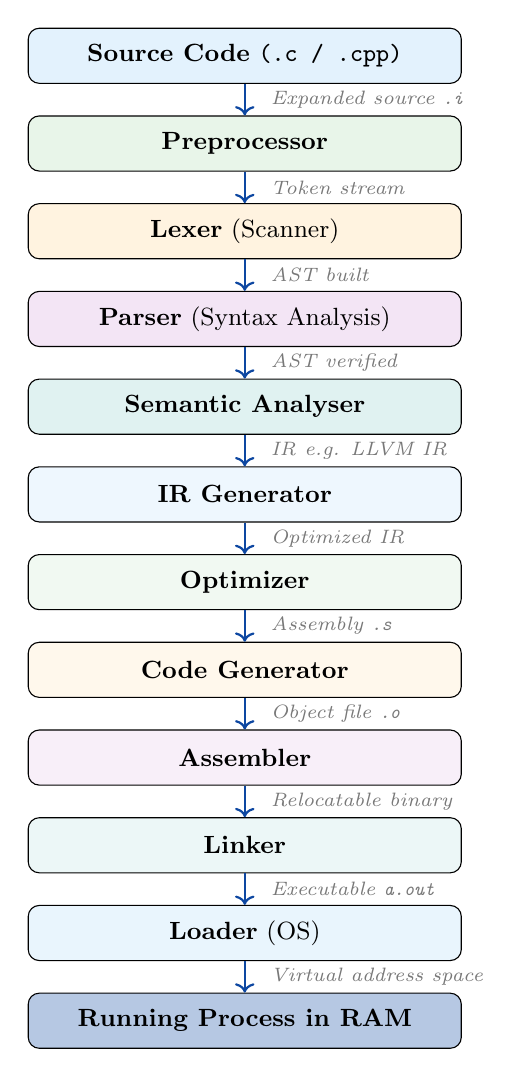
\begin{tikzpicture}[
  font=\small, node distance=0.4cm,
  stage/.style={draw, rounded corners=4pt, fill=#1, minimum width=5.5cm, minimum height=0.7cm, align=center},
  arr/.style={->, thick, darkblue},
  lbl/.style={right=0.2cm, font=\scriptsize\itshape, color=midgray}
]
  \node[stage=lightblue]                        (src)  {\textbf{Source Code} \texttt{(.c / .cpp)}};
  \node[stage=lightgreen, below=of src]         (pre)  {\textbf{Preprocessor}};
  \node[stage=lightorange, below=of pre]        (lex)  {\textbf{Lexer} (Scanner)};
  \node[stage=lightpurple, below=of lex]        (par)  {\textbf{Parser} (Syntax Analysis)};
  \node[stage=lightteal, below=of par]          (sem)  {\textbf{Semantic Analyser}};
  \node[stage=lightblue!60, below=of sem]       (ir)   {\textbf{IR Generator}};
  \node[stage=lightgreen!60, below=of ir]       (opt)  {\textbf{Optimizer}};
  \node[stage=lightorange!60, below=of opt]     (cg)   {\textbf{Code Generator}};
  \node[stage=lightpurple!60, below=of cg]      (as)   {\textbf{Assembler}};
  \node[stage=lightteal!60, below=of as]        (lnk)  {\textbf{Linker}};
  \node[stage=lightblue!80, below=of lnk]       (ldr)  {\textbf{Loader} (OS)};
  \node[stage=darkblue!30, below=of ldr]        (run)  {\textbf{Running Process in RAM}};

  \foreach \a/\b/\t in {
    src/pre/{Expanded source \texttt{.i}},
    pre/lex/{Token stream},
    lex/par/{AST built},
    par/sem/{AST verified},
    sem/ir/{IR e.g. LLVM IR},
    ir/opt/{Optimized IR},
    opt/cg/{Assembly \texttt{.s}},
    cg/as/{Object file \texttt{.o}},
    as/lnk/{Relocatable binary},
    lnk/ldr/{Executable \texttt{a.out}},
    ldr/run/{Virtual address space}
  }{
    \draw[arr] (\a)--(\b) node[lbl, midway]{\t};
  }
\end{tikzpicture}
\end{center}

\subsection{Phase 1: Preprocessor}

\textbf{What it does:} Pure text substitution. Runs BEFORE the compiler sees the code. Knows nothing about C/C++ syntax --- just manipulates text.

\begin{center}
\begin{tabular}{L{4.5cm} L{9cm}}
\toprule
\textbf{Directive} & \textbf{What the Preprocessor Does} \\
\midrule
\code{\#include <stdio.h>} & Copy-pastes the \textit{entire content} of stdio.h at that point in the file \\
\code{\#include "myfile.h"} & Same, but searches current directory first \\
\code{\#define PI 3.14159} & Replaces every \code{PI} token with \code{3.14159} (textual substitution) \\
\code{\#define MAX(a,b) ((a)>(b)?(a):(b))} & Function-like macro (be careful: evaluated multiple times!) \\
\code{\#ifdef DEBUG} & Include following code only if \code{DEBUG} was \code{\#define}d \\
\code{\#ifndef MYHEADER\_H} & Include only if NOT defined (header guard pattern) \\
\code{\#pragma once} & Modern header guard (prevent double inclusion) \\
\code{\#error "message"} & Force a compile error with a message \\
\bottomrule
\end{tabular}
\end{center}

\textbf{Output:} \texttt{.i} file --- a massive plain C file with all includes expanded.\\
\textbf{To see it:} \lstinline[style=bashstyle]{gcc -E main.c -o main.i}

\begin{mcqtrap}
The preprocessor does NOT understand types, functions, or syntax. \code{\#define} is pure text replacement --- it has no type checking! This is why \code{inline} functions or \code{const} variables are preferred over macros in modern C++.
\end{mcqtrap}

\subsection{Phase 2: Lexical Analysis (Lexer / Scanner)}

\textbf{What it does:} Reads the stream of characters from the preprocessed file and groups them into \term{tokens} --- the atomic units of the language.

\textbf{Token Categories:}
\begin{center}
\begin{tabular}{L{3.5cm} L{9.5cm}}
\toprule
\textbf{Token Type} & \textbf{Examples} \\
\midrule
\term{Keywords}      & \code{int}, \code{if}, \code{while}, \code{return}, \code{for}, \code{void}, \code{struct} \\
\term{Identifiers}   & \code{main}, \code{myVariable}, \code{count} (user-defined names) \\
\term{Literals}      & \code{42} (int), \code{3.14} (float), \code{"hello"} (string), \code{'a'} (char) \\
\term{Operators}     & \code{+}, \code{-}, \code{*}, \code{/}, \code{==}, \code{!=}, \code{\&\&}, \code{||} \\
\term{Punctuation}   & \code{\{}, \code{\}}, \code{;}, \code{(}, \code{)}, \code{,} \\
\term{Comments}      & Stripped out completely by lexer \\
\bottomrule
\end{tabular}
\end{center}

\textbf{Implementation:} Uses \term{Regular Expressions} and \term{DFA (Deterministic Finite Automaton)} to recognize patterns.

\textbf{Symbol Table:} During lexing, a symbol table is built: stores all identifier names along with their type, scope, and memory location (filled in later phases).

\begin{myexample}
Input: \code{int x = 5 + 3;}\\
Tokens: \code{[int] [x] [=] [5] [+] [3] [;]}\\
Types:  \code{[keyword] [identifier] [operator] [int-literal] [operator] [int-literal] [punctuation]}
\end{myexample}

\textbf{Errors caught here:} Illegal characters (e.g., \code{\$} in C code outside strings). Note: lexer does NOT catch syntax errors.

\subsection{Phase 3: Syntax Analysis (Parser)}

\textbf{What it does:} Takes the token stream and checks it against the language's \term{grammar} (formally described in BNF or EBNF). Builds an \term{AST (Abstract Syntax Tree)}.

\textbf{Grammar:} A set of rules describing valid programs. For example: \textit{``A statement is an expression followed by a semicolon.'' ``An expression is a term followed by + or - and another term.''} Defined as a \term{Context-Free Grammar (CFG)}.

\textbf{AST for} \code{result = a + b * c;}:
\begin{center}
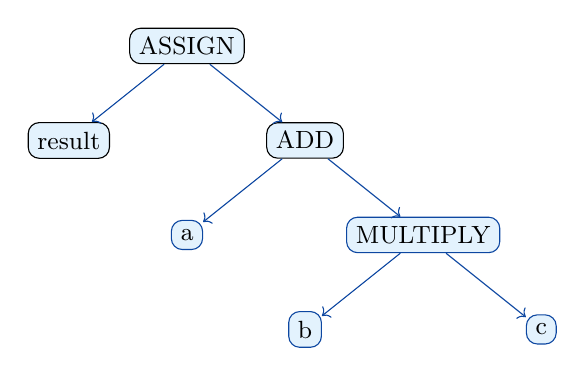
\begin{tikzpicture}[
  level distance=1.2cm, sibling distance=3cm,
  every node/.style={draw, rounded corners, fill=lightblue, font=\small},
  edge from parent/.style={draw, ->, darkblue}
]
\node {ASSIGN}
  child { node {result} }
  child { node {ADD}
    child { node {a} }
    child { node {MULTIPLY}
      child { node {b} }
      child { node {c} }
    }
  };
\end{tikzpicture}
\end{center}

\textbf{Parsing Algorithms:}
\begin{itemize}[noitemsep]
  \item \term{Recursive Descent (Top-Down):} Functions for each grammar rule; call each other recursively. Easy to write by hand. Used in GCC (front end), Clang.
  \item \term{LR Parsing (Bottom-Up):} Uses a parse table (LALR, SLR). More powerful. Used in yacc/bison-generated parsers.
\end{itemize}

\textbf{Syntax errors caught here:}
\begin{itemize}[noitemsep]
  \item \code{int x = ;} $\to$ Missing expression after \code{=}
  \item \code{if x > 5 \{} $\to$ Missing parentheses around condition
  \item \code{int a = (3 + 4;} $\to$ Missing closing parenthesis
\end{itemize}

\subsection{Phase 4: Semantic Analysis}

\textbf{What it does:} Checks that the program is \textit{meaningful}, even if syntactically correct. The AST may be perfectly formed, but the meaning can be wrong.

\textbf{Checks performed:}
\begin{itemize}[noitemsep]
  \item \term{Type Checking:} \code{int x = "hello";} $\to$ Cannot assign string to int. ERROR.
  \item \term{Undeclared Variables:} Using \code{y} without declaring it first. ERROR.
  \item \term{Function Arity:} Calling \code{sqrt(1,2)} when \code{sqrt} takes 1 argument. ERROR.
  \item \term{Scope Resolution:} Variable accessible only in its declared scope.
  \item \term{Array Bounds:} Some compilers warn about obvious out-of-bounds. (Not always caught here.)
  \item \term{Return Type:} Function declared to return \code{int} but body has \code{return "hello";}
\end{itemize}

\begin{myexample}
Syntactically valid but semantically WRONG:
\begin{lstlisting}
int x = 5;
float y = x + "hello";   // type error: cannot add int and char*
int arr[10];
int z = arr;              // type error: array != int
\end{lstlisting}
\end{myexample}

\begin{important}
\textbf{Syntactically valid $\neq$ Semantically valid!}\\
The parser builds the AST regardless of meaning. The semantic analyser checks meaning.
The ANNOTATED AST (with type information attached to each node) is the output of semantic analysis.
\end{important}

\subsection{Phase 5: Intermediate Representation (IR)}

\textbf{Why IR?} The compiler needs a representation that is:
\begin{enumerate}[noitemsep]
  \item High-level enough to analyze and optimize (not assembly)
  \item Low-level enough to generate machine code from
  \item \textbf{Architecture-neutral} so the same front end (C, C++, Rust) can target multiple architectures (x86, ARM, RISC-V)
\end{enumerate}

\begin{center}
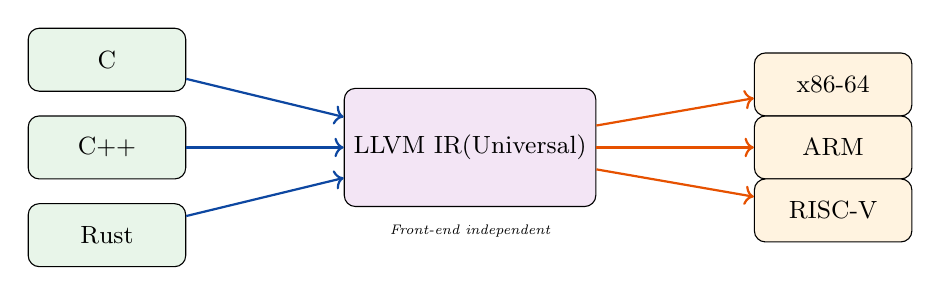
\begin{tikzpicture}[font=\small, node distance=1.5cm]
  \node[draw, fill=lightgreen, rounded corners, minimum width=2cm, minimum height=0.8cm] (c) {C};
  \node[draw, fill=lightgreen, rounded corners, minimum width=2cm, minimum height=0.8cm, below=0.3cm of c] (cpp) {C++};
  \node[draw, fill=lightgreen, rounded corners, minimum width=2cm, minimum height=0.8cm, below=0.3cm of cpp] (rust) {Rust};
  \node[draw, fill=lightpurple, rounded corners, minimum width=2.5cm, minimum height=1.5cm, right=2cm of cpp] (ir) {LLVM IR\\(Universal)};
  \node[draw, fill=lightorange, rounded corners, minimum width=2cm, minimum height=0.8cm, right=2cm of ir, yshift=0.8cm] (x86) {x86-64};
  \node[draw, fill=lightorange, rounded corners, minimum width=2cm, minimum height=0.8cm, right=2cm of ir] (arm) {ARM};
  \node[draw, fill=lightorange, rounded corners, minimum width=2cm, minimum height=0.8cm, right=2cm of ir, yshift=-0.8cm] (rv) {RISC-V};
  \foreach \s in {c,cpp,rust} \draw[->,thick,darkblue] (\s) -- (ir);
  \foreach \t in {x86,arm,rv} \draw[->,thick,orange] (ir) -- (\t);
  \node[below=0.1cm of ir,font=\tiny\itshape]{Front-end independent};
\end{tikzpicture}
\end{center}

\textbf{Common IR Forms:}

\begin{center}
\begin{tabular}{L{4cm} L{9.5cm}}
\toprule
\textbf{IR Form} & \textbf{Description} \\
\midrule
\term{Three-Address Code (TAC)} & At most one operator per statement; at most 3 operands. \code{t1 = a + b; t2 = t1 * c} \\[4pt]
\term{SSA (Static Single Assignment)} & Each variable name is assigned \textit{exactly once}. Makes many optimizations easier. Every assignment creates a new variable version (e.g., \code{x1}, \code{x2}). Used by LLVM and GCC. \\[4pt]
\term{LLVM IR} & Human-readable, strongly-typed IR. Can dump with \lstinline[style=bashstyle]{clang -emit-llvm -S file.c} \\
\bottomrule
\end{tabular}
\end{center}

\subsection{Phase 6: Compiler Optimizations}

Optimizations transform the IR into a semantically equivalent but more efficient version. They are classified as \textbf{machine-independent} (works on any target) or \textbf{machine-dependent} (specific to the target CPU).

\subsubsection{Machine-Independent Optimizations}

\begin{center}
\begin{tabular}{L{5cm} L{8.5cm}}
\toprule
\textbf{Optimization} & \textbf{What It Does} \\
\midrule
\term{Constant Folding} & Evaluate constant expressions at compile time, not runtime. \code{x = 3 * 4 + 2;} $\to$ \code{x = 14;} \\[4pt]
\term{Constant Propagation} & Replace a variable with its known constant value wherever used. \code{int x=5; y=x+3;} $\to$ \code{y=8;} \\[4pt]
\term{Dead Code Elimination} & Remove unreachable or unused code. \code{if(false)\{...\}} removed entirely. Unused variable assignments deleted. \\[4pt]
\term{CSE (Common Subexpression Elimination)} & Compute a repeated sub-expression only once. \code{a=b*c+d; e=b*c+f;} $\to$ compute \code{b*c} once, store in \code{t}. \\[4pt]
\term{Loop Invariant Code Motion (LICM)} & Move computations that don't change across loop iterations to before the loop. \\[4pt]
\term{Loop Unrolling} & Copy the loop body multiple times to reduce loop control overhead (fewer branch checks, better pipelining). \\[4pt]
\term{Function Inlining} & Replace a function call with the body of the function. Eliminates call overhead, enables further optimization. \\[4pt]
\term{Tail Call Optimization (TCO)} & Convert tail-recursive calls into iteration. Prevents stack overflow for deep recursion. \\[4pt]
\term{Strength Reduction} & Replace expensive operations with cheaper equivalents. \code{x * 4} $\to$ \code{x << 2} (shift instead of multiply). \\[4pt]
\term{Loop Fusion} & Combine two adjacent loops over the same range into one (better cache behaviour). \\
\bottomrule
\end{tabular}
\end{center}

\begin{myexample}
\textbf{Loop Invariant Code Motion:}
\begin{lstlisting}
// BEFORE optimization:
for (int i = 0; i < n; i++) {
    result[i] = sin(angle) * arr[i];  // sin(angle) same every iteration!
}

// AFTER optimization:
float temp = sin(angle);    // computed only once, outside loop
for (int i = 0; i < n; i++) {
    result[i] = temp * arr[i];  // now just a multiply per iteration
}
\end{lstlisting}
\end{myexample}

\subsubsection{Machine-Dependent Optimizations}

\begin{itemize}[noitemsep]
  \item \term{Register Allocation:} Decide which variables live in registers (fast) vs memory (slow). Uses \textbf{Graph Coloring algorithm}. Number of available registers is the limit.
  \item \term{Instruction Selection:} Choose the best machine instruction sequence for each IR operation.
  \item \term{Instruction Scheduling:} Reorder machine instructions (while maintaining correctness) to avoid pipeline stalls and fill delay slots.
  \item \term{Peephole Optimization:} Look at a small window (2--5 instructions) and replace with more efficient sequence.
  \item \term{Vectorization (Auto-vectorization):} Convert scalar loops to SIMD instructions (SSE, AVX on x86). E.g., process 8 floats in one AVX instruction instead of 8 separate instructions.
\end{itemize}

\subsubsection{GCC Optimization Flags}

\begin{center}
\begin{tabular}{C{1.5cm} L{11cm}}
\toprule
\textbf{Flag} & \textbf{What It Enables} \\
\midrule
\code{-O0} & No optimization. Every C statement maps directly to assembly. Easiest to debug (default). \\
\code{-O1} & Basic optimizations: constant folding, dead code elimination, CSE, simple inlining. \\
\code{-O2} & \textbf{Standard for production.} Adds: loop invariant motion, more inlining, instruction scheduling, all -O1. \\
\code{-O3} & Aggressive: auto-vectorization, aggressive inlining, loop unrolling. May increase code size. \\
\code{-Os} & Optimize for \textit{code size} (smaller binary). Useful for embedded systems. \\
\code{-Og} & Optimize for debugging experience (some optimization + debuggable). Best for dev+debug. \\
\code{-g}  & Include DWARF debug symbols. Required for GDB. Can combine: \code{-O2 -g}. \\
\code{-Wall} & Enable all important warnings. Always use this! \\
\code{-Wextra} & Even more warnings than \code{-Wall}. \\
\bottomrule
\end{tabular}
\end{center}

\begin{keypoint}
\begin{itemize}[noitemsep]
  \item Development: use \code{-O0 -g -Wall} (no optimization, full debug info, all warnings)
  \item Production: use \code{-O2} (good balance of speed and compile time)
  \item Performance-critical: use \code{-O3} (aggressive, but test carefully)
  \item Embedded: use \code{-Os} (minimize binary size)
\end{itemize}
\end{keypoint}

\subsection{Assembler and Object Files}

The \term{Assembler} converts assembly (\texttt{.s}) to binary machine code (\texttt{.o} / object file).

\textbf{Object file sections:}
\begin{center}
\begin{tabular}{L{2.5cm} L{11cm}}
\toprule
\textbf{Section} & \textbf{Contents} \\
\midrule
\code{.text}   & Machine code (executable instructions) \\
\code{.data}   & Initialized global and static variables (\code{int x = 5;} at global scope) \\
\code{.bss}    & Uninitialized global/static variables (name derived from ``Block Started by Symbol''). Only size stored in file; zeroed at runtime. \\
\code{.rodata} & Read-only data: string literals (\code{"hello"}), \code{const} globals \\
\code{.symtab} & Symbol table: names of functions and variables, whether defined here or external \\
\code{.rel.*}  & Relocation entries: places needing address fixup by linker \\
\bottomrule
\end{tabular}
\end{center}

\begin{keypoint}
Why does \code{.bss} not store actual zeros in the file? Because a 1 MB array of zeros would add 1 MB to the binary file needlessly. Instead, the OS zeroes the memory for free at load time.
\end{keypoint}

\subsection{Linker --- Combining Object Files}

\textbf{The Linker} combines multiple \texttt{.o} files and libraries into a single executable.

\textbf{3 Main Tasks:}
\begin{enumerate}[noitemsep]
  \item \term{Symbol Resolution:} Each \texttt{.o} file may reference symbols (functions, variables) defined in other \texttt{.o} files. The linker matches each undefined reference to its definition. If a symbol is defined nowhere $\to$ ``undefined reference'' error!
  \item \term{Relocation:} In \texttt{.o} files, addresses are relative or placeholder. After merging, the linker knows the final layout, so it patches all addresses to their real values.
  \item \term{Section Merging:} Combine all \code{.text} sections from all \texttt{.o} files into one \code{.text} section, same for \code{.data}, \code{.bss}, etc.
\end{enumerate}

\subsubsection{Static vs Dynamic Linking}

\begin{center}
\begin{tabularx}{\linewidth}{L{3.8cm} X X}
\toprule
\textbf{Aspect} & \textbf{Static Linking} & \textbf{Dynamic Linking} \\
\midrule
What's stored in exe & Full library code COPIED into exe & Just a reference (\textit{stub}) to library \\
When resolved & At link time & At runtime (program launch) \\
Executable size & Large (self-contained) & Small \\
Library update & Must recompile entire program & Just update \texttt{.so}/\texttt{.dll} file; no recompile \\
Library in RAM & Each process has own copy & One copy shared among all processes \\
Startup speed & Slightly faster (no dynamic loading) & Tiny extra overhead for first call \\
Deployment & Simpler (no dependencies) & Target must have library installed \\
Linux library & \texttt{.a} (archive) & \texttt{.so} (shared object) \\
Windows library & \texttt{.lib} & \texttt{.dll} (dynamic link library) \\
Command & \code{gcc -static main.c} & Default on Linux \\
\bottomrule
\end{tabularx}
\end{center}

\textbf{PLT and GOT (Dynamic Linking internals):}
\begin{itemize}[noitemsep]
  \item \term{PLT (Procedure Linkage Table):} A stub for each externally linked function. First call goes to dynamic linker; subsequent calls go directly.
  \item \term{GOT (Global Offset Table):} Stores the actual runtime address of functions/variables from shared libraries. PLT looks up GOT.
\end{itemize}

\subsection{Loader --- Putting the Executable into Memory}

The \term{Loader} is an OS component that runs when you type \code{./myprogram}:

\begin{enumerate}[noitemsep]
  \item Creates a new process (assigns PID, allocates PCB)
  \item Reads the ELF executable header to understand the file layout
  \item Maps \code{.text}, \code{.data}, \code{.bss}, stack, heap into the process's virtual address space using \code{mmap}
  \item For dynamic executables: invokes the \textbf{dynamic linker} (\code{ld.so}) to load and link shared libraries
  \item Sets up the initial stack (command-line arguments \code{argc/argv}, environment variables)
  \item Jumps to the entry point: \code{\_start} (provided by C runtime libc), which calls \code{main()}
\end{enumerate}

\textbf{ELF (Executable and Linkable Format):} Standard binary format on Linux for executables, \texttt{.so}, and \texttt{.o} files.\\
\textbf{PE (Portable Executable):} Windows equivalent.

\begin{mcqtrap}
\begin{itemize}[noitemsep]
  \item ``Which produces a larger binary?'' $\to$ \highlight{Static linking}
  \item ``Library update without recompile?'' $\to$ \highlight{Dynamic linking}
  \item ``Linker vs Loader?'' $\to$ Linker runs at COMPILE time. Loader runs at PROGRAM LAUNCH.
  \item ``\texttt{.bss} section stores?'' $\to$ \highlight{Uninitialized global/static variables} (NOT their actual values)
  \item ``\texttt{.so} vs \texttt{.a}?'' $\to$ \texttt{.so} = shared (dynamic). \texttt{.a} = archive (static).
  \item ``What is PLT?'' $\to$ \highlight{Procedure Linkage Table} for dynamic function call resolution
\end{itemize}
\end{mcqtrap}

%% ================================================================
\section{Profiling and Debugging}
%% ================================================================

\subsection{GDB --- GNU Debugger (Deep Dive)}

\begin{mydef}
\textbf{GDB:} A source-level debugger that lets you run a program interactively, pause it at specific points, inspect memory and variables, and understand why it's crashing.
\end{mydef}

\textbf{ALWAYS compile with \code{-g}:}
\begin{lstlisting}[style=bashstyle]
gcc -g -O0 main.c -o main_debug   # -g: debug symbols, -O0: no optimization
gdb ./main_debug                   # launch GDB
\end{lstlisting}

Why \code{-O0}? With optimization, the compiler reorders/eliminates code, making debugging confusing. Variables may be ``optimized out.''

\subsubsection{Complete GDB Command Reference}

\begin{center}
\begin{longtable}{L{5cm} L{9cm}}
\toprule
\textbf{Command} & \textbf{What It Does} \\
\midrule
\code{run [args]} & Start the program (with optional args). \\
\code{break main} & Set breakpoint at the start of function \code{main}. \\
\code{break file.c:42} & Set breakpoint at line 42 of file.c. \\
\code{break *0x4007a2} & Set breakpoint at an absolute address (for assembly debugging). \\
\code{tbreak func} & Temporary breakpoint: fires once, then deleted. \\
\code{watch var} & Watchpoint: pause whenever variable \code{var} changes value. \\
\code{rwatch var} & Read watchpoint: pause whenever \code{var} is read. \\
\code{catch signal SIGSEGV} & Pause when SIGSEGV (segfault) occurs, before crash. \\
\code{next} / \code{n} & Execute next source line; step OVER function calls. \\
\code{step} / \code{s} & Execute next source line; step INTO function calls. \\
\code{nexti} & Execute next \textit{assembly} instruction, step over. \\
\code{stepi} & Execute next \textit{assembly} instruction, step into. \\
\code{continue} / \code{c} & Continue execution until next breakpoint. \\
\code{finish} & Run until current function returns; print return value. \\
\code{until 50} & Continue until line 50 is reached. \\
\code{print x} / \code{p x} & Print current value of variable \code{x}. \\
\code{p *ptr} & Dereference and print the pointer. \\
\code{p arr[0]@10} & Print 10 elements of array starting at \code{arr[0]}. \\
\code{display x} & Auto-print \code{x} after every step (unlike \code{print} which is manual). \\
\code{info locals} & Show all local variables in current frame. \\
\code{info args} & Show function arguments in current frame. \\
\code{info registers} & Show all CPU register values. \\
\code{backtrace} / \code{bt} & Show full call stack. \\
\code{bt full} & Call stack with local variables of each frame. \\
\code{frame N} & Switch to stack frame N (0 = current). \\
\code{up} / \code{down} & Move up/down one frame in the call stack. \\
\code{list} & Show source code around current line. \\
\code{disassemble func} & Show assembly of function \code{func}. \\
\code{x/10xw 0xaddr} & Examine 10 words in hex at address. \\
\code{set var x = 5} & Change variable \code{x} to 5 while debugging! \\
\code{condition 1 x > 100} & Make breakpoint 1 fire only when \code{x > 100}. \\
\code{ignore 1 5} & Skip breakpoint 1 the next 5 times it's hit. \\
\code{info breakpoints} & List all breakpoints with their numbers. \\
\code{delete 1} & Delete breakpoint 1. \\
\code{disable 2} & Temporarily disable breakpoint 2. \\
\code{enable 2} & Re-enable breakpoint 2. \\
\code{quit} / \code{q} & Exit GDB. \\
\bottomrule
\end{longtable}
\end{center}

\subsubsection{Stack Frame and Backtrace --- Understanding Crashes}

Every function call creates a \term{stack frame} pushed onto the call stack. It contains:
\begin{itemize}[noitemsep]
  \item Local variables of that function
  \item Return address (where execution resumes after the function returns)
  \item Saved registers (so callee can restore them)
  \item Parameters passed to the function
\end{itemize}

\begin{myexample}
\textbf{Backtrace of a segfault:}
\begin{lstlisting}[style=bashstyle]
Program received signal SIGSEGV, Segmentation fault.
0x00000000004005a2 in write_to_null () at main.c:8

(gdb) backtrace
#0  write_to_null () at main.c:8
#1  0x00000000004005d1 in process_data (data=0x0) at main.c:20
#2  0x0000000000400612 in main () at main.c:35

(gdb) frame 1
#1  process_data (data=0x0) at main.c:20   # data pointer is NULL!
(gdb) p data
$1 = (int *) 0x0    # Confirmed: null pointer passed!
\end{lstlisting}
Read bottom-up: \code{main} called \code{process\_data} with a NULL pointer, which called \code{write\_to\_null}, which crashed. The bug is: \code{main} passing NULL.
\end{myexample}

\subsubsection{Core Dumps --- Post-Mortem Analysis}

A \term{core dump} is a snapshot of the process's memory at the moment of crash. Think of it as a freeze-frame photograph of the crash scene.

\begin{lstlisting}[style=bashstyle]
# Step 1: Enable core dumps (disabled by default on many systems)
ulimit -c unlimited           # allow core files of unlimited size
echo "core.%p" | sudo tee /proc/sys/kernel/core_pattern  # name pattern

# Step 2: Run the program (it crashes)
./buggy_program               # crash! Produces 'core' or 'core.1234'

# Step 3: Analyze the core dump
gdb ./buggy_program core      # load the crash snapshot
(gdb) backtrace               # see exactly where it crashed
(gdb) info locals             # see variable values AT TIME OF CRASH
\end{lstlisting}

Core dumps allow debugging crashes that:
\begin{itemize}[noitemsep]
  \item Happen in production (can't attach GDB interactively)
  \item Are hard to reproduce
  \item Happen in CI/CD pipelines
\end{itemize}

%% -------------------------------------------------------------------
\subsection{Valgrind --- Memory Error Detection}
%% -------------------------------------------------------------------

\begin{mydef}
\textbf{Valgrind:} A suite of dynamic analysis tools. The default tool \textit{memcheck} instruments EVERY memory operation at runtime, detecting all kinds of memory errors. \textbf{Overhead: 10--50x slower.}
\end{mydef}

\begin{analogy}
Valgrind is like a safety inspector who follows every worker (memory operation) around, checking if they're using the right tools in the right places. Very thorough, but the inspection slows everything down.
\end{analogy}

\begin{lstlisting}[style=bashstyle]
valgrind ./program                          # basic (memcheck)
valgrind --leak-check=full ./program        # detailed leak report
valgrind --leak-check=full --show-leak-kinds=all ./program  # even more detail
valgrind --track-origins=yes ./program      # track where uninitialized values came from
\end{lstlisting}

\subsubsection{What Valgrind Memcheck Detects}

\begin{center}
\begin{tabular}{L{4.5cm} L{4cm} L{5cm}}
\toprule
\textbf{Error Type} & \textbf{C Code Causing It} & \textbf{Danger} \\
\midrule
\term{Memory Leak} & \code{malloc()} without \code{free()} & Memory consumed until crash \\[4pt]
\term{Heap Buffer Overflow} & \code{arr[n+5] = 1;} (past end) & Corrupts adjacent memory \\[4pt]
\term{Stack Buffer Overflow} & \code{char buf[10]; buf[15]='a'} & Corrupts return address $\to$ crash or exploit \\[4pt]
\term{Use After Free} & \code{free(p); p->x = 5;} & Undefined behavior \\[4pt]
\term{Double Free} & \code{free(p); free(p);} & Heap corruption \\[4pt]
\term{Uninitialized Read} & \code{int x; if(x>0)\{..\}} & Random behavior \\
\bottomrule
\end{tabular}
\end{center}

\subsubsection{Reading Valgrind Output}

\begin{lstlisting}[style=bashstyle]
==12345== Invalid read of size 4
==12345==    at 0x401234: main (main.c:15)
==12345==  Address 0x5204060 is 4 bytes after a block of size 40 alloc'd
==12345==    at 0x4C2FB0F: malloc (in /usr/lib/valgrind/vgpreload_memcheck)
==12345==    by 0x401210: main (main.c:12)
\end{lstlisting}
\textbf{Reading:} At main.c line 15, you read 4 bytes past the end of a 40-byte block allocated at line 12. Classic off-by-one error: \code{malloc(10 * sizeof(int))} then accessed \code{arr[10]}.

\begin{lstlisting}[style=bashstyle]
==12345== LEAK SUMMARY:
==12345==    definitely lost: 40 bytes in 1 blocks    # definitely leaked
==12345==    indirectly lost: 0 bytes in 0 blocks     # leaked through ptr to lost block
==12345==      possibly lost: 0 bytes in 0 blocks     # suspicious
==12345==    still reachable: 128 bytes in 3 blocks   # pointer exists but not freed (often ok)
\end{lstlisting}

\subsubsection{Valgrind Tools}

\begin{center}
\begin{tabular}{L{4cm} L{9cm}}
\toprule
\textbf{Tool} & \textbf{Purpose} \\
\midrule
\code{memcheck} (default) & Memory errors, leaks, uninitialized reads \\
\code{callgrind} & Instruction-level profiling, call graph with exact counts \\
\code{cachegrind} & Cache and branch prediction simulation \\
\code{massif} & Heap memory profiling over time (peak heap usage) \\
\code{helgrind} & Thread error detection (race conditions, lock order violations) \\
\code{DRD} & Data race detection (alternative to helgrind) \\
\bottomrule
\end{tabular}
\end{center}

\begin{lstlisting}[style=bashstyle]
valgrind --tool=callgrind ./program    # profiling
valgrind --tool=massif ./program       # heap profiling
valgrind --tool=helgrind ./program     # race conditions
\end{lstlisting}

%% -------------------------------------------------------------------
\subsection{Sanitizers --- Compile-Time Instrumentation}
%% -------------------------------------------------------------------

\begin{mydef}
\textbf{Sanitizers:} Compiler tools that add checking code directly into your binary at compile time. Much faster than Valgrind ($\sim$2x overhead) because the checks are native code, not a virtual machine.
\end{mydef}

\begin{center}
\begin{tabular}{L{4.5cm} L{5cm} L{4cm}}
\toprule
\textbf{Sanitizer} & \textbf{Flag} & \textbf{Detects} \\
\midrule
\term{AddressSanitizer (ASan)} & \code{-fsanitize=address} & Heap/stack/global buffer overflow, use-after-free, double-free \\[4pt]
\term{ThreadSanitizer (TSan)} & \code{-fsanitize=thread} & Data races between threads \\[4pt]
\term{UndefinedBehaviorSanitizer (UBSan)} & \code{-fsanitize=undefined} & Signed int overflow, null deref, misaligned access, div-by-zero \\[4pt]
\term{MemorySanitizer (MSan)} & \code{-fsanitize=memory} & Reads from uninitialized memory (Clang only) \\[4pt]
\term{LeakSanitizer (LSan)} & \code{-fsanitize=leak} & Memory leaks (built into ASan) \\
\bottomrule
\end{tabular}
\end{center}

\begin{lstlisting}[style=bashstyle]
# Compile and run with ASan (detects memory errors instantly):
gcc -fsanitize=address -g main.c -o main_asan
./main_asan
# On error: prints detailed report with stack trace and immediately aborts

# Detect race conditions:
gcc -fsanitize=thread -g main.c -o main_tsan -lpthread
./main_tsan

# Detect undefined behavior:
gcc -fsanitize=undefined -g main.c -o main_ubsan
./main_ubsan

# Combine multiple sanitizers (ASan + UBSan):
gcc -fsanitize=address,undefined -g main.c -o main
\end{lstlisting}

\textbf{ASan Output Example:}
\begin{lstlisting}[style=bashstyle]
=================================================================
==1234==ERROR: AddressSanitizer: heap-buffer-overflow on address 0x602000000028
READ of size 4 at 0x602000000028 thread T0
    #0 0x4008d2 in main main.c:15
    ...
0x602000000028 is located 8 bytes after a region of size 40 alloc'd
    #0 0x7faa in __interceptor_malloc
    #1 0x40087c in main main.c:10
\end{lstlisting}

\begin{keypoint}
\textbf{Valgrind vs Sanitizers comparison:}
\begin{center}
\begin{tabular}{L{4cm} C{3cm} C{3cm} C{3cm}}
\toprule
& \textbf{Valgrind} & \textbf{ASan} & \textbf{TSan} \\
\midrule
Compilation needed & No & Yes & Yes \\
Overhead & 10--50x & $\sim$2x & $\sim$5--10x \\
Memory overhead & 1--2x & 2--3x & 5--10x \\
Works without source & Yes & No & No \\
Coverage & Very thorough & High & Data races only \\
\bottomrule
\end{tabular}
\end{center}
\end{keypoint}

%% -------------------------------------------------------------------
\subsection{Profiling --- Finding Performance Bottlenecks}
%% -------------------------------------------------------------------

\begin{mydef}
\textbf{Profiling:} Measuring a program's runtime behavior --- which functions consume the most CPU time, how many times each is called, cache behavior, etc. Goal: find the ``hot spot'' (20\% of code taking 80\% of time).
\end{mydef}

\begin{analogy}
Profiling is like a time-and-motion study in a factory: you observe every worker (function) to find out who is spending too much time and why.
\end{analogy}

\textbf{Two main approaches:}
\begin{itemize}[noitemsep]
  \item \term{Sampling Profiler:} Periodically interrupts the program (e.g., every 1 ms) and records the current Program Counter. Statistical approximation, very low overhead ($<$5\%).
  \item \term{Instrumentation Profiler:} Adds code at every function entry/exit to measure exact call counts and time. Accurate but higher overhead ($\sim$30--100\%).
\end{itemize}

\subsubsection{gprof --- Classic Instrumentation Profiler}

\begin{lstlisting}[style=bashstyle]
gcc -pg -O2 main.c -o main     # -pg inserts profiling hooks
./main                          # run your program; produces gmon.out
gprof ./main gmon.out > report.txt
cat report.txt
\end{lstlisting}

\textbf{Flat Profile output (most important part):}
\begin{lstlisting}[style=bashstyle]
  %   cumulative   self              self     total
 time   seconds   seconds    calls  ms/call  ms/call  name
 78.4      2.35     2.35       10   235.0    235.0  matrix_multiply
 15.2      2.81     0.46    10000     0.046    0.046  process_element
  6.4      3.00     0.19        1   190.0    190.0  load_data
\end{lstlisting}

\code{matrix\_multiply} uses 78.4\% of the time! This is the optimization target.

\subsubsection{perf --- Linux Hardware Performance Counter Profiler}

Modern, sampling-based, very low overhead. Uses hardware performance counters built into CPUs.

\begin{lstlisting}[style=bashstyle]
# Summary statistics:
perf stat ./program
# Output includes:
#   1,234,567,890  cycles
#     987,654,321  instructions   # IPC = instructions / cycles
#     234,567,890  cache-misses   # high = cache inefficient
#          12,345  branch-misses  # high = branch prediction failing

# Record samples for detailed analysis:
perf record -g ./program         # -g = include call graph
perf report                      # interactive TUI showing hot functions
perf annotate slow_function      # show which assembly instructions are hot
perf top                         # live profiling (like 'top' for CPU)
\end{lstlisting}

\textbf{Key perf stats to watch:}
\begin{itemize}[noitemsep]
  \item \textbf{IPC (Instructions Per Cycle) $<$ 1:} CPU is stalling frequently (cache misses, branch mispredictions)
  \item \textbf{Cache miss rate $>$ 5\%:} Memory access pattern is cache-unfriendly
  \item \textbf{Branch miss rate $>$ 5\%:} Branches are hard to predict; consider branchless code
\end{itemize}

\subsubsection{Static Analysis Tools}

Find bugs \textit{without running} the program (compile time or post-compile):

\begin{center}
\begin{tabular}{L{4cm} L{10cm}}
\toprule
\textbf{Tool} & \textbf{What It Finds} \\
\midrule
\code{clang --analyze} & Null pointer dereference, memory leak paths, logic errors via symbolic execution \\
\code{cppcheck} & C/C++ bugs: array overflows, uninitialized vars, style issues. \code{cppcheck --enable=all src/} \\
\code{Coverity} & Commercial; very deep analysis; used in industry \\
\code{SonarQube} & Multi-language; CI/CD integration; security vulnerabilities \\
\code{Splint} & Annotation-based C checker (older) \\
\bottomrule
\end{tabular}
\end{center}

\begin{mcqtrap}
\begin{itemize}[noitemsep]
  \item ``Lower overhead: Valgrind or ASan?'' $\to$ \highlight{ASan} ($\sim$2x vs 10--50x)
  \item ``Detects race conditions?'' $\to$ \highlight{TSan} or Valgrind helgrind
  \item ``No recompile needed?'' $\to$ \highlight{Valgrind} (works on any binary)
  \item ``Detects uninitialized memory reads (Clang only)?'' $\to$ \highlight{MSan (MemorySanitizer)}
  \item ``gprof uses which profiling approach?'' $\to$ \highlight{Instrumentation}
  \item ``perf uses which approach?'' $\to$ \highlight{Sampling} (hardware counters)
\end{itemize}
\end{mcqtrap}

%% ================================================================
\section{Parallel Programming}
%% ================================================================

\subsection{Processes vs Threads --- The Foundation}

\subsubsection{Process}

\begin{mydef}
\textbf{Process:} An independent program in execution, with its own virtual address space, file descriptors, and OS resources. Processes are isolated from each other --- one process cannot directly read/write another's memory.
\end{mydef}

\textbf{A process has its OWN:}
\begin{itemize}[noitemsep]
  \item Virtual address space (code, stack, heap, data segments)
  \item File descriptor table (open files, sockets)
  \item PID (Process ID)
  \item Signal handlers
  \item Page table
\end{itemize}

\textbf{Creating a process:} \code{fork()} in Unix/Linux duplicates the calling process. The new process is called the \textit{child}. They start as identical copies, then diverge.

\subsubsection{Thread}

\begin{mydef}
\textbf{Thread:} A lightweight execution unit \textit{within} a process. Multiple threads in the same process share most of the process's resources but each has its own execution context.
\end{mydef}

\textbf{All threads in a process SHARE:}
\begin{itemize}[noitemsep]
  \item Code segment (\code{.text})
  \item Global and static variables (\code{.data}, \code{.bss})
  \item Heap memory
  \item File descriptors
  \item Signal handlers, process ID
\end{itemize}

\textbf{Each thread has its OWN:}
\begin{itemize}[noitemsep]
  \item Stack (local variables, function call chain)
  \item Registers (including Program Counter)
  \item Thread ID
  \item TLS (Thread-Local Storage): variables declared \code{\_\_thread int x;}
\end{itemize}

\begin{center}
\begin{tabular}{L{5cm} C{3cm} C{3cm}}
\toprule
\textbf{Aspect} & \textbf{Process} & \textbf{Thread} \\
\midrule
Memory isolation & Complete & None (shared) \\
Creation cost & High ($\sim$ms) & Low ($\sim$$\mu$s) \\
Context switch & Expensive (TLB flush) & Cheaper (same page table) \\
Communication & IPC (pipes, sockets, shmem) & Shared memory directly \\
Crash isolation & One crash doesn't affect others & One crash kills all threads \\
\bottomrule
\end{tabular}
\end{center}

\subsubsection{Context Switch}

When the OS switches the CPU from one process/thread to another:
\begin{enumerate}[noitemsep]
  \item Save CPU state of running task (registers, PC, stack pointer) to its PCB/TCB
  \item Load CPU state of next task
  \item For process switch: also switch page tables (TLB must be flushed or tagged with ASID)
  \item Resume execution of next task
\end{enumerate}

\textbf{Why thread context switch is cheaper:} Threads within the same process share the page table, so no TLB flush is needed when switching between threads of the same process.

%% -------------------------------------------------------------------
\subsection{POSIX Threads (pthreads) --- Complete Guide}
%% -------------------------------------------------------------------

\subsubsection{Thread Lifecycle}

\begin{lstlisting}
#include <pthread.h>
#include <stdio.h>

// Thread function: must take void* and return void*
void* thread_function(void* arg) {
    int my_id = *(int*)arg;
    printf("Thread %d: starting work\n", my_id);
    // ... do work ...
    printf("Thread %d: done\n", my_id);
    return (void*)(long)42;  // return value (optional)
}

int main() {
    pthread_t thread1, thread2;
    int id1 = 1, id2 = 2;
    
    // Create threads
    pthread_create(&thread1, NULL, thread_function, &id1);
    pthread_create(&thread2, NULL, thread_function, &id2);
    
    // Wait for threads to finish
    void* retval;
    pthread_join(thread1, &retval);  // blocks until thread1 exits
    printf("Thread 1 returned: %ld\n", (long)retval);
    pthread_join(thread2, NULL);     // NULL = don't care about return
    
    return 0;
}
// Compile: gcc -pthread main.c -o main
\end{lstlisting}

\subsubsection{Mutex --- Mutual Exclusion Lock}

\begin{mydef}
\textbf{Mutex:} A synchronization primitive that ensures only ONE thread executes a critical section at a time. A thread \textit{acquires} (locks) the mutex before the critical section and \textit{releases} (unlocks) after.
\end{mydef}

\textbf{Why do we need it?} Even a simple \code{counter++} is NOT atomic. It compiles to 3 machine instructions: LOAD (read counter from memory), INCREMENT (add 1 to register), STORE (write back). Two threads can interleave these operations and lose increments!

\begin{lstlisting}
pthread_mutex_t my_lock;        // declare mutex
pthread_mutex_init(&my_lock, NULL);   // initialize

// --- or use static initializer: ---
pthread_mutex_t my_lock = PTHREAD_MUTEX_INITIALIZER;

void* increment_counter(void* arg) {
    for (int i = 0; i < 100000; i++) {
        pthread_mutex_lock(&my_lock);    // ACQUIRE lock (blocks if locked)
        counter++;                        // critical section: safe!
        pthread_mutex_unlock(&my_lock);  // RELEASE lock (wakes up waiters)
    }
    return NULL;
}
// At end: pthread_mutex_destroy(&my_lock);
\end{lstlisting}

\textbf{Types of Mutex:}
\begin{itemize}[noitemsep]
  \item \term{Normal:} Default. Locking twice from same thread = deadlock.
  \item \term{Recursive:} Same thread can lock multiple times (must unlock same number of times).
  \item \term{Error-checking:} Returns error instead of deadlock on double-lock.
\end{itemize}

\subsubsection{Semaphore --- Counting Synchronization}

\begin{mydef}
\textbf{Semaphore:} A non-negative integer counter with two atomic operations: \code{wait()} (decrement; block if 0) and \code{post()} (increment; wake a waiter).
\end{mydef}

\begin{lstlisting}
#include <semaphore.h>

sem_t my_sem;
sem_init(&my_sem, 0, 3);   // initial value = 3 (allows 3 concurrent accesses)

// Thread trying to access resource:
sem_wait(&my_sem);    // decrement; if 0, block until someone posts
// --- access resource (up to 3 threads simultaneously) ---
sem_post(&my_sem);    // increment; wake one waiter if any

sem_destroy(&my_sem);
\end{lstlisting}

\textbf{Binary semaphore (value 0 or 1) works like a mutex BUT with a key difference:}

\begin{center}
\begin{tabular}{L{5cm} L{4.5cm} L{4.5cm}}
\toprule
& \textbf{Mutex} & \textbf{Semaphore} \\
\midrule
Ownership & Yes: only locker can unlock & No: any thread can post \\
Value range & Binary (locked/unlocked) & $0, 1, 2, ..., N$ \\
Use case & Protecting shared data & Signaling + resource counting \\
Priority inheritance & Supported & Not typically \\
Best for & Mutual exclusion & Producer-consumer signaling \\
\bottomrule
\end{tabular}
\end{center}

\subsubsection{Condition Variable --- Waiting for a Condition}

\begin{mydef}
\textbf{Condition Variable:} Allows threads to block (sleep) until some condition becomes true, while atomically releasing a mutex. Used in producer-consumer, bounded buffer, etc.
\end{mydef}

\begin{lstlisting}
// Classic Producer-Consumer with condition variable:
pthread_mutex_t lock = PTHREAD_MUTEX_INITIALIZER;
pthread_cond_t  not_empty = PTHREAD_COND_INITIALIZER;
pthread_cond_t  not_full  = PTHREAD_COND_INITIALIZER;
int queue[10], head=0, tail=0, count=0;

void* producer(void* arg) {
    int item = produce_item();
    pthread_mutex_lock(&lock);
    while (count == 10) {               // queue is full; wait
        pthread_cond_wait(&not_full, &lock);  // release lock, sleep
    }
    queue[tail] = item;
    tail = (tail + 1) % 10;
    count++;
    pthread_cond_signal(&not_empty);    // wake one consumer
    pthread_mutex_unlock(&lock);
    return NULL;
}

void* consumer(void* arg) {
    pthread_mutex_lock(&lock);
    while (count == 0) {                // queue is empty; wait
        pthread_cond_wait(&not_empty, &lock);
    }
    int item = queue[head];
    head = (head + 1) % 10;
    count--;
    pthread_cond_signal(&not_full);     // wake one producer
    pthread_mutex_unlock(&lock);
    consume_item(item);
    return NULL;
}
\end{lstlisting}

\textbf{Critical Rules for Condition Variables:}
\begin{enumerate}[noitemsep]
  \item \textbf{ALWAYS use \code{while} not \code{if}!} Due to \term{spurious wakeups}, a thread can wake up even without being signaled. The \code{while} re-checks the condition.
  \item Mutex must be held before calling \code{pthread\_cond\_wait}.
  \item \code{pthread\_cond\_wait} atomically releases the mutex and blocks.
  \item On waking, \code{pthread\_cond\_wait} re-acquires the mutex before returning.
\end{enumerate}

%% -------------------------------------------------------------------
\subsection{Concurrency Problems --- Detailed Analysis}
%% -------------------------------------------------------------------

\subsubsection{Race Condition}

\begin{mydef}
\textbf{Race Condition:} When multiple threads access shared data concurrently and the final result depends on the timing/order of execution. The program gives different results on different runs.
\end{mydef}

\begin{myexample}
Without mutex, two threads each incrementing a counter 100,000 times often give a result less than 200,000 because both read the old value, increment, and write back --- losing some increments.

Timeline of a lost update:
\begin{lstlisting}[style=bashstyle]
Time  Thread 1                Thread 2     counter value
  1   LOAD counter -> reg1                 counter = 5
  2   (reg1 = 5)              LOAD -> reg2  counter = 5
  3                           (reg2 = 5)
  4   reg1 = reg1 + 1
  5   (reg1 = 6)
  6                           reg2 = reg2 + 1  (reg2 = 6)
  7   STORE reg1 -> counter                counter = 6 (not 7!)
  8                           STORE reg2   counter = 6 (lost one!)
\end{lstlisting}
\end{myexample}

\subsubsection{Deadlock --- Complete Analysis}

\begin{mydef}
\textbf{Deadlock:} A state where two or more threads are each waiting for a resource held by another thread in the set. Nobody can proceed. The system is stuck permanently.
\end{mydef}

\textbf{The Four Coffman Conditions --- ALL must hold simultaneously for deadlock:}

\begin{center}
\begin{tabular}{L{4cm} L{9cm}}
\toprule
\textbf{Condition} & \textbf{Meaning} \\
\midrule
\term{1. Mutual Exclusion} & Resources cannot be shared; only one thread can hold a resource at a time \\[4pt]
\term{2. Hold and Wait} & A thread holds at least one resource AND is waiting to acquire additional resources \\[4pt]
\term{3. No Preemption} & Resources cannot be forcibly taken from a thread; only voluntarily released \\[4pt]
\term{4. Circular Wait} & A circular chain exists: Thread 1 waits for T2's lock, T2 waits for T1's lock \\
\bottomrule
\end{tabular}
\end{center}

\textbf{Classic Deadlock --- Dining Philosophers variant:}
\begin{lstlisting}
pthread_mutex_t lockA, lockB;

void* thread1(void* arg) {
    pthread_mutex_lock(&lockA);    // Thread 1 grabs A
    sleep(1);
    pthread_mutex_lock(&lockB);    // Thread 1 waits for B (held by Thread 2)
    // ... Thread 1 STUCK FOREVER
}

void* thread2(void* arg) {
    pthread_mutex_lock(&lockB);    // Thread 2 grabs B
    sleep(1);
    pthread_mutex_lock(&lockA);    // Thread 2 waits for A (held by Thread 1)
    // ... Thread 2 STUCK FOREVER
}
\end{lstlisting}

\textbf{Deadlock Prevention Strategies:}

\begin{center}
\begin{tabular}{L{4.5cm} L{9cm}}
\toprule
\textbf{Strategy} & \textbf{How It Works} \\
\midrule
\term{Lock Ordering} & Always acquire locks in a globally consistent order (e.g., always lock A before B). Breaks circular wait. \\[4pt]
\term{Try-Lock with Timeout} & Use \code{pthread\_mutex\_trylock()}: if can't get lock immediately, release all held locks and retry later. \\[4pt]
\term{Resource Pre-allocation} & Acquire ALL needed locks before starting. Breaks hold-and-wait. \\[4pt]
\term{Deadlock Detection + Recovery} & OS builds a wait-for graph periodically; detects cycles; kills one thread to break cycle. \\[4pt]
\term{Lock-Free Data Structures} & Use atomic operations (CAS: Compare-And-Swap) instead of locks. No locks = no deadlock. \\
\bottomrule
\end{tabular}
\end{center}

\subsubsection{Livelock}

\begin{mydef}
\textbf{Livelock:} Threads are NOT blocked (they keep running and consuming CPU), but they keep changing state in response to each other without making any progress toward completion.
\end{mydef}

\begin{analogy}
Two people meet in a narrow corridor. Person A steps right to let Person B pass. Person B steps right at the same moment. Now they're still blocking each other. A steps left. B steps left. Repeat forever. Both are ``active'' but going nowhere.
\end{analogy}

\textbf{Example:} Two threads detect a conflict and both ``politely back off'' --- but they back off, check for the other, and try again at the exact same moment, forever.

\subsubsection{Starvation}

\begin{mydef}
\textbf{Starvation:} A thread is perpetually denied the CPU or a lock because other threads (usually higher priority) always get preference. The thread never completes.
\end{mydef}

\textbf{Example:} In a priority-based scheduler, a low-priority thread waits for a lock forever because high-priority threads always preempt before it gets the lock.

\textbf{Solution:} \term{Aging} --- gradually increase the priority of a waiting thread over time. Eventually it becomes high priority and gets the lock.

\begin{keypoint}
\textbf{Three concurrency problems compared:}
\begin{itemize}[noitemsep]
  \item \textbf{Deadlock:} All involved threads are BLOCKED, waiting forever. System must kill/restart.
  \item \textbf{Livelock:} Threads are RUNNING actively, consuming CPU, but making no progress. Harder to detect!
  \item \textbf{Starvation:} ONE thread never gets to run. Others are fine. Solution: fairness/aging.
\end{itemize}
\end{keypoint}

%% -------------------------------------------------------------------
\subsection{OpenMP --- Shared Memory Parallel Programming}
%% -------------------------------------------------------------------

\begin{mydef}
\textbf{OpenMP:} An API for shared-memory parallel programming using compiler directives (\code{\#pragma omp}), library routines, and environment variables. Works on multi-core CPUs within a single machine.
\end{mydef}

\begin{lstlisting}[style=bashstyle]
gcc -fopenmp main.c -o main    # must link with OpenMP
export OMP_NUM_THREADS=8       # set number of threads (or use omp_set_num_threads())
\end{lstlisting}

\subsubsection{Core OpenMP Constructs}

\begin{lstlisting}
#include <omp.h>
#include <stdio.h>

int main() {
    // ---- Parallel Region: all threads execute this block ----
    #pragma omp parallel
    {
        int tid = omp_get_thread_num();
        int total = omp_get_num_threads();
        printf("Hello from thread %d of %d\n", tid, total);
    }  // implicit barrier: all threads join here

    // ---- Parallel For: divide loop iterations among threads ----
    int n = 1000;
    double a[1000], b[1000], c[1000];
    #pragma omp parallel for
    for (int i = 0; i < n; i++) {
        c[i] = a[i] + b[i];   // each thread handles a chunk of i values
    }

    // ---- Reduction: safe parallel sum/product/min/max ----
    double sum = 0.0;
    #pragma omp parallel for reduction(+:sum)
    for (int i = 0; i < n; i++) {
        sum += a[i];    // each thread has private sum; merged at end
    }
    printf("Sum = %f\n", sum);

    // ---- Critical Section: only one thread at a time ----
    #pragma omp parallel
    {
        #pragma omp critical
        {
            global_count++;  // safe, but serialized!
        }
    }

    // ---- Barrier: all threads must reach here before any continue ----
    #pragma omp parallel
    {
        do_phase_one();
        #pragma omp barrier   // synchronize all threads
        do_phase_two();       // only starts after ALL threads finish phase one
    }

    // ---- Single: only ONE thread executes this block ----
    #pragma omp parallel
    {
        do_parallel_work();
        #pragma omp single
        {
            printf("Only one thread prints this\n");
        }
        // implicit barrier after single
    }

    // ---- Master: only the MASTER (thread 0) executes this ----
    #pragma omp parallel
    {
        #pragma omp master
        {
            printf("I am thread 0, the master\n");
        }
        // NO implicit barrier after master!
    }
    return 0;
}
\end{lstlisting}

\subsubsection{Variable Scoping --- shared vs private}

\begin{lstlisting}
int x = 10;
int result = 0;

#pragma omp parallel for private(x) shared(result)
for (int i = 0; i < n; i++) {
    x = compute(i);       // each thread has its own x (uninitialized!)
    result += x;          // DANGER: result is shared, race condition!
}

// Correct way: use reduction for result
#pragma omp parallel for private(x) reduction(+:result)
for (int i = 0; i < n; i++) {
    x = compute(i);
    result += x;           // safe with reduction
}
\end{lstlisting}

\begin{center}
\begin{tabular}{L{3cm} L{11cm}}
\toprule
\textbf{Clause} & \textbf{Meaning} \\
\midrule
\code{shared(x)} & All threads share the same \code{x}. Must synchronize if writing! \\
\code{private(x)} & Each thread gets its own uninitialized copy of \code{x}. \\
\code{firstprivate(x)} & Each thread gets a copy initialized with the value of \code{x} from before the region. \\
\code{lastprivate(x)} & After region, \code{x} has the value from the last iteration. \\
\code{reduction(op:x)} & Each thread has private copy; all are combined with \code{op} at end. ops: \code{+}, \code{*}, \code{min}, \code{max}, \code{\&\&}, \code{||} \\
\bottomrule
\end{tabular}
\end{center}

\subsubsection{Scheduling Strategies}

\begin{center}
\begin{tabular}{L{4cm} L{9.5cm}}
\toprule
\textbf{Schedule} & \textbf{How Iterations Are Distributed} \\
\midrule
\code{schedule(static)} & Divide iterations into equal-sized chunks; assign round-robin upfront. Predictable. \\
\code{schedule(static,k)} & Chunks of size k, assigned round-robin. \\
\code{schedule(dynamic)} & Each idle thread grabs the next iteration. Best for uneven workloads. Higher overhead. \\
\code{schedule(dynamic,k)} & Each idle thread grabs k iterations at a time. \\
\code{schedule(guided)} & Large chunks first, halving each time. Good trade-off. \\
\code{schedule(runtime)} & Determined by \code{OMP\_SCHEDULE} env variable at runtime. \\
\bottomrule
\end{tabular}
\end{center}

%% -------------------------------------------------------------------
\subsection{MPI --- Distributed Memory Programming}
%% -------------------------------------------------------------------

\begin{mydef}
\textbf{MPI (Message Passing Interface):} A standard library for parallel programs running on separate processes (no shared memory). Processes communicate by explicitly sending and receiving messages. Can span multiple machines over a network.
\end{mydef}

\textbf{Key terminology:}
\begin{itemize}[noitemsep]
  \item \term{Rank:} Unique integer ID of each MPI process (0 to N-1)
  \item \term{Communicator:} Group of processes. \code{MPI\_COMM\_WORLD} = all processes
  \item \term{Point-to-Point:} One process $\to$ one other process
  \item \term{Collective:} All processes in a communicator participate simultaneously
\end{itemize}

\subsubsection{Basic MPI Program}

\begin{lstlisting}
#include <mpi.h>
#include <stdio.h>

int main(int argc, char** argv) {
    MPI_Init(&argc, &argv);       // initialize MPI environment

    int rank, size;
    MPI_Comm_rank(MPI_COMM_WORLD, &rank);   // get MY rank
    MPI_Comm_size(MPI_COMM_WORLD, &size);   // get total number of processes

    printf("Process %d of %d: Hello!\n", rank, size);

    MPI_Finalize();   // clean up MPI
    return 0;
}
\end{lstlisting}
\begin{lstlisting}[style=bashstyle]
mpicc main.c -o main         # compile
mpirun -np 4 ./main          # run with 4 processes
mpirun -np 8 -host n1,n2 ./main  # 8 processes across 2 machines!
\end{lstlisting}

\subsubsection{Point-to-Point Communication}

\begin{lstlisting}
// MPI_Send signature:
// MPI_Send(buf, count, datatype, dest_rank, tag, communicator)
// MPI_Recv signature:
// MPI_Recv(buf, count, datatype, src_rank, tag, communicator, &status)

if (rank == 0) {
    int data[100];
    // ... fill data ...
    MPI_Send(data, 100, MPI_INT, 1, 42, MPI_COMM_WORLD);
    // Blocks until data is buffered or received by rank 1
    printf("Rank 0: sent data\n");
} else if (rank == 1) {
    int data[100];
    MPI_Status status;
    MPI_Recv(data, 100, MPI_INT, 0, 42, MPI_COMM_WORLD, &status);
    // Blocks until message from rank 0 with tag 42 arrives
    printf("Rank 1: received %d elements\n", status.MPI_SOURCE);
}
\end{lstlisting}

\textbf{Non-blocking communication (overlap compute + communicate):}
\begin{lstlisting}
MPI_Request req;
MPI_Isend(data, 100, MPI_INT, 1, 0, MPI_COMM_WORLD, &req);
// Returns immediately! Data transfer happens in background.
do_useful_computation();       // CPU does other work while data transfers
MPI_Wait(&req, MPI_STATUS_IGNORE);   // ensure send is complete before reusing buffer
\end{lstlisting}

\subsubsection{Collective Operations --- All Processes Participate}

\begin{center}
\begin{tabular}{L{3.5cm} L{10cm}}
\toprule
\textbf{Function} & \textbf{What It Does} \\
\midrule
\code{MPI\_Bcast} & Rank 0 (root) sends same data to ALL processes \\
\code{MPI\_Scatter} & Root sends different chunks of an array to each process \\
\code{MPI\_Gather} & Each process sends chunk; root collects them all into one array \\
\code{MPI\_Allgather} & Like Gather, but ALL processes get the complete result \\
\code{MPI\_Reduce} & Each process contributes; result (sum/max/etc.) at root \\
\code{MPI\_Allreduce} & Like Reduce, but ALL processes get the result \\
\code{MPI\_Barrier} & All processes wait until all have called this \\
\code{MPI\_Scan} & Prefix sum: each process gets sum of ranks 0..its rank \\
\bottomrule
\end{tabular}
\end{center}

\begin{lstlisting}
// Example: parallel sum across all processes
double local_sum = compute_local_part(rank, size);
double global_sum;
MPI_Allreduce(&local_sum, &global_sum, 1, MPI_DOUBLE,
              MPI_SUM, MPI_COMM_WORLD);
// Now ALL processes have global_sum
\end{lstlisting}

\begin{mcqtrap}
\begin{itemize}[noitemsep]
  \item ``OpenMP works on?'' $\to$ \highlight{Shared memory, single machine, threads}
  \item ``MPI works on?'' $\to$ \highlight{Distributed memory, can span multiple machines, processes}
  \item ``MPI\_Send is?'' $\to$ \highlight{Blocking} (MPI\_Isend = non-blocking)
  \item ``Which MPI collective gives result to ALL?'' $\to$ \highlight{MPI\_Allreduce, MPI\_Allgather}
  \item ``Spurious wakeup means?'' $\to$ \highlight{Condition variable wakeup without signal; use while not if}
  \item ``Coffman conditions: how many?'' $\to$ \highlight{4: ME, Hold\&Wait, No Preemption, Circular Wait}
\end{itemize}
\end{mcqtrap}

%% -------------------------------------------------------------------
\subsection{Amdahl's Law \& Gustafson's Law --- Detailed}
%% -------------------------------------------------------------------

\subsubsection{Amdahl's Law}

\begin{mydef}
\textbf{Amdahl's Law:} The theoretical maximum speedup of a program when parallelized, given that some fraction of it must remain serial.
\end{mydef}

Let:
\begin{itemize}[noitemsep]
  \item $P$ = fraction of program that is parallelizable ($0 \leq P \leq 1$)
  \item $(1-P)$ = serial fraction
  \item $N$ = number of processors
\end{itemize}

\[
\boxed{S(N) = \frac{1}{(1-P) + \dfrac{P}{N}}} \qquad\qquad S_{\max} = \lim_{N\to\infty} S(N) = \frac{1}{1-P}
\]

\textbf{Worked Example Table ($P = 0.9$, i.e., 90\% parallelizable):}

\begin{center}
\begin{tabular}{C{3cm} C{3cm} C{3cm}}
\toprule
\textbf{Processors (N)} & \textbf{Speedup} & \textbf{Efficiency (S/N)} \\
\midrule
1     & 1.00$\times$  & 100\% \\
2     & 1.82$\times$  & 91\% \\
4     & 3.08$\times$  & 77\% \\
10    & 5.26$\times$  & 53\% \\
100   & 9.17$\times$  & 9.2\% \\
1000  & 9.91$\times$  & 1.0\% \\
$\infty$ & \textbf{10$\times$ maximum!} & $\approx$0\% \\
\bottomrule
\end{tabular}
\end{center}

\textbf{Key Insight:} Even with 90\% parallel code, you can NEVER exceed $1/(1-0.9) = 10\times$ speedup no matter how many CPUs you add. The serial 10\% is the absolute bottleneck.

\textbf{Corollary:} If 5\% of code is serial ($1-P = 0.05$), max speedup = $1/0.05 = \mathbf{20}\times$. Adding 1000 CPUs won't help beyond 20$\times$!

\subsubsection{Gustafson's Law}

\begin{mydef}
\textbf{Gustafson's Law:} Amdahl assumes fixed problem size. In practice, we often scale the problem with more processors. Gustafson says speedup can be nearly linear if the workload scales.
\end{mydef}

\[
\boxed{S(N) = N - \alpha(N-1)} \qquad \alpha = \text{serial fraction}
\]

\textbf{Example:} $\alpha = 0.05$ (5\% serial), $N = 100$ processors:\\
$S(100) = 100 - 0.05 \times 99 = 100 - 4.95 = \mathbf{95.05}\times$

\textbf{Key Difference from Amdahl:} Gustafson fixes the time (not the problem size). With more processors, you solve a bigger problem in the same time $\to$ near-linear speedup.

\begin{keypoint}
\textbf{Amdahl:} Pessimistic. Fixed problem size. Serial bottleneck limits speedup hard.\\
\textbf{Gustafson:} Optimistic. Scaled problem size. Near-linear speedup is achievable in practice.\\
\textbf{Real world:} Both apply depending on the use case.
\end{keypoint}

%% ================================================================
\section{Heterogeneous Computing --- CPU-GPU Interaction}
%% ================================================================

\subsection{Why GPUs? --- The Fundamental Difference}

\begin{analogy}
CPU = 8 experts (complex, flexible, independent). GPU = 10,000 assembly line workers (simple, repetitive, all doing the same thing). For sorting a complex database: use the experts. For adding 1 to a billion numbers: use the assembly line.
\end{analogy}

\begin{center}
\begin{tabular}{L{4cm} L{4.5cm} L{5cm}}
\toprule
\textbf{Feature} & \textbf{CPU} & \textbf{GPU} \\
\midrule
Optimized for & \textbf{Latency} (do one thing fast) & \textbf{Throughput} (do many things) \\
Core count & 8--64 powerful cores & 1,000s--10,000s simple cores \\
Clock speed & High (3--5 GHz) & Lower (1--2 GHz) \\
Cache & Large (MBs, smart) & Small (designed for bandwidth) \\
Branch prediction & Sophisticated (95\%+) & Minimal \\
Memory & System RAM (GBs, shared) & VRAM (GBs, high-bandwidth) \\
Memory bandwidth & $\sim$50--100 GB/s & $\sim$500--3000 GB/s \\
Best for & OS, databases, sequential code & Matrix ops, image/video, ML training \\
\bottomrule
\end{tabular}
\end{center}

\subsection{GPU Architecture --- NVIDIA CUDA}

\subsubsection{Hardware Hierarchy}

\begin{center}
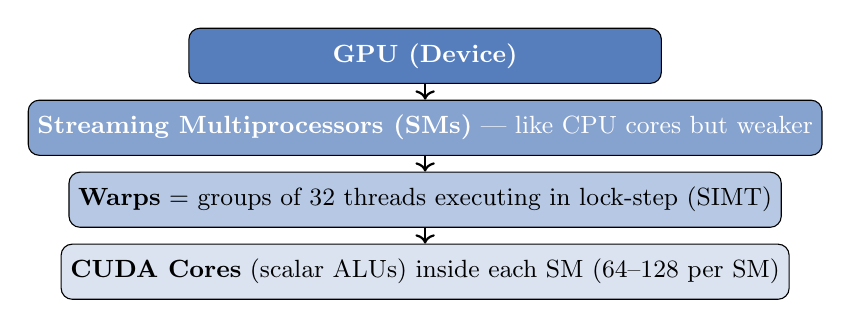
\begin{tikzpicture}[font=\small,
  box/.style={draw,rounded corners,fill=#1,minimum width=6cm,minimum height=0.7cm,align=center}
]
  \node[box=darkblue!70,text=white] (gpu) {\textbf{GPU (Device)}};
  \node[box=darkblue!50,text=white, below=0.2cm of gpu] (sm) {\textbf{Streaming Multiprocessors (SMs)} --- like CPU cores but weaker};
  \node[box=darkblue!30, below=0.2cm of sm] (warp) {\textbf{Warps} = groups of 32 threads executing in lock-step (SIMT)};
  \node[box=darkblue!15, below=0.2cm of warp] (cu) {\textbf{CUDA Cores} (scalar ALUs) inside each SM (64--128 per SM)};
  \draw[->,thick] (gpu)--(sm); \draw[->,thick] (sm)--(warp); \draw[->,thick] (warp)--(cu);
\end{tikzpicture}
\end{center}

\textbf{Typical GPU numbers (NVIDIA A100):}
\begin{itemize}[noitemsep]
  \item 108 SMs $\times$ 64 CUDA cores = 6,912 CUDA cores total
  \item 80 GB VRAM, 2,039 GB/s memory bandwidth
  \item 312 TFLOPS for FP16 operations
\end{itemize}

\subsubsection{SIMT --- Single Instruction, Multiple Threads}

GPUs use \term{SIMT} execution: all 32 threads in a \term{warp} execute the SAME instruction at the SAME time, but each on DIFFERENT data. This is the GPU's way of doing SIMD (Single Instruction, Multiple Data) with threads.

\textbf{Warp:} The fundamental scheduling unit on NVIDIA GPUs. \textbf{Warp size = 32 threads}. The SM always schedules and executes 32 threads together.

\textbf{AMD equivalent:} \term{Wavefront} = 64 threads (same concept).

\subsubsection{Warp Divergence --- Critical Performance Issue}

\begin{mydef}
\textbf{Warp Divergence:} When threads within a warp take different execution paths (due to if-else or switch), the GPU serializes the paths --- first executes one branch with some threads active, then the other branch with the remaining threads active.
\end{mydef}

\begin{lstlisting}
// BAD: divergence within warp (threads have different threadIdx.x values)
__global__ void bad_kernel(int* a) {
    if (threadIdx.x % 2 == 0) {      // even threads take if-branch
        a[threadIdx.x] *= 2;          // odd threads IDLE here
    } else {
        a[threadIdx.x] += 10;         // even threads IDLE here
    }
    // RESULT: warp takes TWICE as long as it should!
}

// GOOD: no divergence (all threads in a warp take the same path)
__global__ void good_kernel(int* a, int n) {
    int i = blockIdx.x * blockDim.x + threadIdx.x;
    if (i < n) {      // all threads either ALL in bounds or ALL out (usually)
        a[i] += 1;    // no divergence within warp
    }
}
\end{lstlisting}

\textbf{Why is it bad?} A warp has 32 threads. With 50\% divergence (half take if, half take else): the warp now needs to execute BOTH branches serially $\to$ throughput drops to 50\%. At worst (32 different paths): 1/32 = 3\% throughput!

\begin{keypoint}
Minimize branching that depends on \code{threadIdx.x} or thread-specific values within a warp. If divergence is unavoidable, try to structure code so threads in the SAME warp always take the SAME branch.
\end{keypoint}

%% -------------------------------------------------------------------
\subsection{CUDA Programming Model --- Complete Guide}
%% -------------------------------------------------------------------

\subsubsection{Execution Hierarchy --- Grid, Block, Thread}

\begin{center}
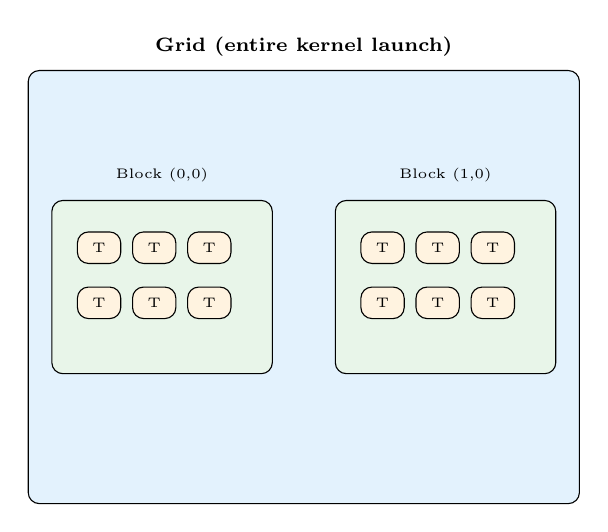
\begin{tikzpicture}[font=\small,
  box/.style={draw,rounded corners,fill=#1,minimum width=2cm,minimum height=0.8cm,align=center}
]
  \node[box=lightblue, minimum width=7cm, minimum height=5.5cm] (grid) {};
  \node[above=0.05cm of grid.north, font=\scriptsize\bfseries] {Grid (entire kernel launch)};

  \node[box=lightgreen, minimum width=2.8cm, minimum height=2.2cm] at ([xshift=-1.8cm]grid.center) (b0) {};
  \node[above=0.1cm of b0.north, font=\tiny] {Block (0,0)};
  \node[box=lightgreen, minimum width=2.8cm, minimum height=2.2cm] at ([xshift=1.8cm]grid.center) (b1) {};
  \node[above=0.1cm of b1.north, font=\tiny] {Block (1,0)};

  \foreach \x/\y in {-0.8/0.5,-0.1/0.5,0.6/0.5,-0.8/-0.2,-0.1/-0.2,0.6/-0.2} {
    \node[box=lightorange, minimum width=0.55cm, minimum height=0.4cm, font=\tiny] at ([xshift=\x cm, yshift=\y cm]b0.center) {T};
  }
  \foreach \x/\y in {-0.8/0.5,-0.1/0.5,0.6/0.5,-0.8/-0.2,-0.1/-0.2,0.6/-0.2} {
    \node[box=lightorange, minimum width=0.55cm, minimum height=0.4cm, font=\tiny] at ([xshift=\x cm, yshift=\y cm]b1.center) {T};
  }
\end{tikzpicture}
\end{center}

\begin{center}
\begin{tabular}{L{3.5cm} L{10cm}}
\toprule
\textbf{Unit} & \textbf{Description} \\
\midrule
\term{Thread} & Smallest execution unit. Runs one instance of the kernel function. \\
\term{Block (Thread Block)} & Group of threads (up to 1024). Threads in a block can share data via \textbf{shared memory} and synchronize via \code{\_\_syncthreads()}. Assigned to ONE SM. \\
\term{Grid} & Collection of all blocks for one kernel launch. Blocks are distributed across SMs. No direct communication between blocks (within one kernel). \\
\term{Warp} & 32 consecutive threads from a block, grouped by hardware for SIMT execution. \\
\bottomrule
\end{tabular}
\end{center}

\subsubsection{Thread Indexing --- Most Important for MCQs}

Built-in variables available inside every kernel:

\begin{center}
\begin{tabular}{L{4cm} L{9cm}}
\toprule
\textbf{Variable} & \textbf{Meaning} \\
\midrule
\code{threadIdx.x / .y / .z} & Thread's index \textit{within its block} (x, y, z dimensions) \\
\code{blockIdx.x / .y / .z}  & Block's index \textit{within the grid} \\
\code{blockDim.x / .y / .z}  & Number of threads \textit{per block} (same for all blocks) \\
\code{gridDim.x / .y / .z}   & Number of blocks \textit{in the grid} \\
\bottomrule
\end{tabular}
\end{center}

\textbf{Computing the unique global thread ID:}
\[
\boxed{\text{globalID} = \texttt{blockIdx.x} \times \texttt{blockDim.x} + \texttt{threadIdx.x}}
\]

\begin{myexample}
Grid has 4 blocks, each block has 256 threads.\\
Total threads = $4 \times 256 = 1024$.\\
For thread 15 in block 3: globalID $= 3 \times 256 + 15 = 783$.\\
For thread 0 in block 0: globalID $= 0 \times 256 + 0 = 0$.\\
For thread 255 in block 3: globalID $= 3 \times 256 + 255 = 1023$.\\
\textbf{Formula for number of blocks:} $\lceil N / \text{threadsPerBlock} \rceil = (N + \text{tpb} - 1) / \text{tpb}$
\end{myexample}

\textbf{2D thread indexing (for matrix operations):}
\begin{lstlisting}
// 2D grid and block
dim3 blockDim(16, 16);    // 16x16 = 256 threads per block
dim3 gridDim((N+15)/16, (M+15)/16);   // enough blocks for N x M matrix

__global__ void matAdd(float* A, float* B, float* C, int N, int M) {
    int row = blockIdx.y * blockDim.y + threadIdx.y;
    int col = blockIdx.x * blockDim.x + threadIdx.x;
    if (row < M && col < N) {
        C[row * N + col] = A[row * N + col] + B[row * N + col];
    }
}
\end{lstlisting}

\subsubsection{Complete CUDA Program --- Vector Addition}

\begin{lstlisting}
#include <cuda_runtime.h>
#include <stdio.h>

// ---- GPU Kernel (runs on device, called from host) ----
__global__ void vectorAdd(float* A, float* B, float* C, int N) {
    int i = blockIdx.x * blockDim.x + threadIdx.x;  // global thread ID
    if (i < N) {          // ALWAYS check boundary (N may not be divisible by blockDim)
        C[i] = A[i] + B[i];
    }
}

int main() {
    int N = 1 << 20;   // 1M elements
    size_t bytes = N * sizeof(float);

    // ---- Host memory (CPU/RAM) ----
    float *h_A = (float*)malloc(bytes);
    float *h_B = (float*)malloc(bytes);
    float *h_C = (float*)malloc(bytes);
    for (int i = 0; i < N; i++) { h_A[i] = 1.0f; h_B[i] = 2.0f; }

    // ---- Device memory (GPU/VRAM) ----
    float *d_A, *d_B, *d_C;
    cudaMalloc(&d_A, bytes);   // allocate on GPU
    cudaMalloc(&d_B, bytes);
    cudaMalloc(&d_C, bytes);

    // ---- Copy data: Host -> Device ----
    cudaMemcpy(d_A, h_A, bytes, cudaMemcpyHostToDevice);
    cudaMemcpy(d_B, h_B, bytes, cudaMemcpyHostToDevice);

    // ---- Launch kernel ----
    int threadsPerBlock = 256;
    int blocksPerGrid = (N + threadsPerBlock - 1) / threadsPerBlock; // ceil(N/256)
    printf("Launching %d blocks of %d threads\n", blocksPerGrid, threadsPerBlock);
    vectorAdd<<<blocksPerGrid, threadsPerBlock>>>(d_A, d_B, d_C, N);

    // ---- Check for kernel errors ----
    cudaError_t err = cudaGetLastError();
    if (err != cudaSuccess) printf("Kernel error: %s\n", cudaGetErrorString(err));

    // ---- Copy result: Device -> Host ----
    cudaMemcpy(h_C, d_C, bytes, cudaMemcpyDeviceToHost);

    // Verify
    printf("C[0] = %f (expected 3.0)\n", h_C[0]);

    // ---- Free memory ----
    cudaFree(d_A); cudaFree(d_B); cudaFree(d_C);
    free(h_A); free(h_B); free(h_C);
    return 0;
}
// Compile: nvcc vectorAdd.cu -o vectorAdd
\end{lstlisting}

%% -------------------------------------------------------------------
\subsection{GPU Memory Types --- Complete Reference}
%% -------------------------------------------------------------------

\begin{center}
\begin{tabular}{L{3cm} C{2cm} L{2.5cm} L{2.5cm} L{2cm} L{2cm}}
\toprule
\textbf{Type} & \textbf{Location} & \textbf{Scope} & \textbf{Lifetime} & \textbf{Speed} & \textbf{Size} \\
\midrule
Registers & On-chip & Per-thread & Thread & Fastest & $\sim$255/thread \\
Shared Memory & On-chip & Per-block & Block & Very fast & 48--96 KB/SM \\
Local Memory & VRAM (off-chip) & Per-thread & Thread & Slow & Large \\
Global Memory & VRAM (off-chip) & All threads & Program & Slow & GBs \\
Constant Memory & VRAM + cache & All threads & Program & Fast (read-only) & 64 KB \\
Texture Memory & VRAM + cache & All threads & Program & Spatial caching & VRAM size \\
\bottomrule
\end{tabular}
\end{center}

\subsubsection{Registers}
\begin{itemize}[noitemsep]
  \item Fastest memory; completely private to each thread
  \item Compiler automatically allocates kernel variables to registers
  \item \term{Register Spilling:} If a kernel uses too many registers ($>$255), extras spill to \textbf{Local Memory} (which is actually VRAM --- much slower!)
  \item Too many registers $\to$ fewer active threads on SM $\to$ lower occupancy $\to$ worse latency hiding
\end{itemize}

\subsubsection{Shared Memory}
\begin{itemize}[noitemsep]
  \item On-chip SRAM: very fast ($\sim$same speed as L1 cache)
  \item Shared among all threads in the SAME block
  \item Programmer-managed: must explicitly declare and load/store
  \item 48 KB -- 96 KB per SM (configurable: can trade vs L1 cache)
  \item Used for: inter-thread communication within a block, tiling/blocking for cache optimization
\end{itemize}

\begin{lstlisting}
__global__ void dotProduct(float* A, float* B, float* result, int N) {
    __shared__ float partial[256];   // shared among all 256 threads in block
    int i = blockIdx.x * blockDim.x + threadIdx.x;

    // Each thread computes its partial product and stores in shared memory
    partial[threadIdx.x] = (i < N) ? A[i] * B[i] : 0.0f;
    __syncthreads();    // WAIT: all threads must finish loading before we reduce

    // Parallel reduction within block using shared memory
    for (int stride = blockDim.x/2; stride > 0; stride /= 2) {
        if (threadIdx.x < stride)
            partial[threadIdx.x] += partial[threadIdx.x + stride];
        __syncthreads();    // sync at every reduction step
    }
    if (threadIdx.x == 0)
        atomicAdd(result, partial[0]);   // add block result to global result
}
\end{lstlisting}

\subsubsection{Global Memory}
\begin{itemize}[noitemsep]
  \item Main GPU VRAM. Large (GBs). Accessible by all threads in all blocks.
  \item Slowest GPU memory (hundreds of cycles latency)
  \item \textbf{Memory coalescing} is critical for performance (see below)
  \item Most data lives here (input/output arrays passed to kernels)
\end{itemize}

\subsubsection{Local Memory}
\begin{itemize}[noitemsep]
  \item Confusingly named: ``local'' means private to the thread, NOT that it's on-chip
  \item Physically in global memory (VRAM) --- just as slow
  \item Used for: register spills, large arrays inside kernels, complex structs
  \item Automatically used by compiler when needed (you don't declare it)
\end{itemize}

\subsubsection{Constant Memory}
\begin{itemize}[noitemsep]
  \item 64 KB, read-only from device, writable from host (\code{cudaMemcpyToSymbol})
  \item Cached: when all threads in a warp read the SAME address, served from cache (1 transaction)
  \item Best for: lookup tables, model weights, parameters that all threads read
\end{itemize}

\begin{lstlisting}
__constant__ float weights[1024];  // in constant memory (declared at file scope)

// On host:
cudaMemcpyToSymbol(weights, h_weights, 1024 * sizeof(float));
\end{lstlisting}

%% -------------------------------------------------------------------
\subsection{Memory Coalescing --- Critical Optimization}
%% -------------------------------------------------------------------

\begin{mydef}
\textbf{Memory Coalescing:} When multiple threads in a warp access global memory, the GPU can combine (coalesce) multiple requests into a single memory transaction IF the accesses are contiguous and aligned.
\end{mydef}

\begin{analogy}
Think of 32 people each needing to pick up a package from a warehouse. If their packages are on the same shelf (contiguous), one truck trip picks them all up. If their packages are in 32 different warehouses, 32 trips are needed.
\end{analogy}

\begin{center}
\begin{tabular}{L{5cm} L{4.5cm} L{4cm}}
\toprule
\textbf{Access Pattern} & \textbf{Code} & \textbf{Transactions} \\
\midrule
\term{Coalesced} (best) & \code{a[threadIdx.x]} & 1 transaction for 32 threads \\
Stride-2 & \code{a[2*threadIdx.x]} & 2 transactions \\
Stride-32 & \code{a[32*threadIdx.x]} & 32 transactions \\
\term{Random} (worst) & \code{a[random[threadIdx.x]]} & Up to 32 transactions \\
\bottomrule
\end{tabular}
\end{center}

\begin{lstlisting}
// COALESCED (fast): thread i accesses element i
__global__ void coalesced(float* a, int n) {
    int i = blockIdx.x * blockDim.x + threadIdx.x;
    if (i < n) a[i] *= 2;   // threads 0,1,...,31 access a[0],a[1],...,a[31]
                              // hardware coalesces into ONE 128-byte transaction
}

// NON-COALESCED (slow): threads access strided locations
__global__ void strided(float* a, int n) {
    int i = (blockIdx.x * blockDim.x + threadIdx.x) * 32;  // stride of 32
    if (i < n) a[i] *= 2;   // threads access a[0],a[32],a[64],...,a[992]
                              // 32 separate 4-byte transactions!
}

// NON-COALESCED (slow): transposed matrix access
// When accessing matrix column-by-column (row-major storage):
__global__ void bad_transpose(float* mat, int rows, int cols) {
    int row = blockIdx.x * blockDim.x + threadIdx.x;
    // threads in warp access mat[0][col], mat[1][col], ... = strided!
    float val = mat[row * cols + blockIdx.y];  // column access = bad coalescing
}
\end{lstlisting}

\begin{keypoint}
\textbf{Rule:} Thread $i$ should access element $i$ in global memory arrays. Design data layout and access patterns so that consecutive threads (same warp) access consecutive memory addresses.
\end{keypoint}

%% -------------------------------------------------------------------
\subsection{Data Movement --- CPU-GPU Communication}
%% -------------------------------------------------------------------

\subsubsection{PCIe Bus Bandwidth}

Data between CPU RAM and GPU VRAM travels over the PCIe bus:
\begin{center}
\begin{tabular}{L{4cm} C{3cm} C{3cm}}
\toprule
\textbf{PCIe Version} & \textbf{x16 Bandwidth} & \textbf{Bidirectional} \\
\midrule
PCIe 3.0 & $\sim$16 GB/s & $\sim$32 GB/s \\
PCIe 4.0 & $\sim$32 GB/s & $\sim$64 GB/s \\
PCIe 5.0 & $\sim$64 GB/s & $\sim$128 GB/s \\
NVLink (A100) & \multicolumn{2}{c}{$\sim$600 GB/s (GPU-to-GPU)} \\
\bottomrule
\end{tabular}
\end{center}

\textbf{Critical: GPU memory bandwidth vs PCIe bandwidth:}
\begin{itemize}[noitemsep]
  \item NVIDIA A100 GPU memory bandwidth: $\sim$2,039 GB/s
  \item PCIe 4.0 $\times$16: $\sim$32 GB/s
  \item \textbf{GPU-to-GPU memory is $\sim$64$\times$ faster than CPU-to-GPU!}
  \item \textbf{Implication: minimize host-to-device transfers. Keep data on GPU as long as possible.}
\end{itemize}

\subsubsection{cudaMemcpy Variants}

\begin{lstlisting}
// Synchronous (blocking) transfers:
cudaMemcpy(d_dst, h_src, bytes, cudaMemcpyHostToDevice);   // CPU RAM -> GPU VRAM
cudaMemcpy(h_dst, d_src, bytes, cudaMemcpyDeviceToHost);   // GPU VRAM -> CPU RAM
cudaMemcpy(d_dst, d_src, bytes, cudaMemcpyDeviceToDevice); // GPU -> GPU (within same GPU)

// Pinned (page-locked) host memory: ~2x faster transfers
float* h_pinned;
cudaMallocHost(&h_pinned, bytes);   // allocate pinned memory on host
// use h_pinned for transfers
cudaFreeHost(h_pinned);

// Unified Memory: single pointer, auto-migrated between CPU and GPU
float* unified;
cudaMallocManaged(&unified, bytes);   // accessible from both host and device
// use unified on CPU
// launch kernel using unified on GPU (CUDA runtime migrates pages automatically)
cudaDeviceSynchronize();
// use unified on CPU again (migrated back)
cudaFree(unified);
\end{lstlisting}

\textbf{Pinned vs Pageable Memory:}
\begin{itemize}[noitemsep]
  \item \term{Pageable memory} (normal malloc): OS can swap it to disk. DMA can't work directly $\to$ CUDA internally copies to a pinned buffer first (double copy).
  \item \term{Pinned memory} (cudaMallocHost): Locked in physical RAM, never swapped. DMA works directly $\to$ faster transfer. But pinned memory is limited; using too much hurts OS performance.
\end{itemize}

\subsubsection{Asynchronous Transfers --- Overlapping Compute and Transfer}

\begin{lstlisting}
cudaStream_t stream1, stream2;
cudaStreamCreate(&stream1);
cudaStreamCreate(&stream2);

// Strategy: pipeline compute and transfer using multiple streams
float *d_in1, *d_out1, *d_in2, *d_out2;
cudaMalloc(&d_in1, bytes/2); cudaMalloc(&d_in2, bytes/2);
cudaMalloc(&d_out1, bytes/2); cudaMalloc(&d_out2, bytes/2);

// Stream 1: transfer first half while stream 2 processes second half
cudaMemcpyAsync(d_in1, h_in, bytes/2, cudaMemcpyHostToDevice, stream1);
cudaMemcpyAsync(d_in2, h_in+N/2, bytes/2, cudaMemcpyHostToDevice, stream2);

myKernel<<<blocks, threads, 0, stream1>>>(d_in1, d_out1, N/2);
myKernel<<<blocks, threads, 0, stream2>>>(d_in2, d_out2, N/2);

cudaMemcpyAsync(h_out, d_out1, bytes/2, cudaMemcpyDeviceToHost, stream1);
cudaMemcpyAsync(h_out+N/2, d_out2, bytes/2, cudaMemcpyDeviceToHost, stream2);

cudaStreamSynchronize(stream1);
cudaStreamSynchronize(stream2);
\end{lstlisting}

%% -------------------------------------------------------------------
\subsection{CUDA Synchronization --- Complete Guide}
%% -------------------------------------------------------------------

\subsubsection{Synchronization Levels}

\begin{center}
\begin{tabular}{L{5cm} L{9cm}}
\toprule
\textbf{Synchronization} & \textbf{What It Does} \\
\midrule
\code{\_\_syncthreads()} & Synchronizes all threads within the SAME block. ALL threads must reach this before any can proceed. Device-side (inside kernel). \\[4pt]
\code{cudaDeviceSynchronize()} & CPU waits until ALL GPU operations (all streams) complete. Host-side. \\[4pt]
\code{cudaStreamSynchronize(s)} & CPU waits until all operations in stream \code{s} complete. Host-side. \\[4pt]
\code{cudaEventSynchronize(e)} & CPU waits until a specific event is recorded on GPU. \\[4pt]
\code{atomicAdd()} etc. & Atomic operations for single variables within global/shared memory. Thread-safe. \\
\bottomrule
\end{tabular}
\end{center}

\subsubsection{\_\_syncthreads() --- Rules and Pitfalls}

\begin{lstlisting}
__global__ void reduction_kernel(float* data, float* result) {
    __shared__ float smem[256];
    int tid = threadIdx.x;
    int i = blockIdx.x * blockDim.x + tid;

    smem[tid] = data[i];        // load from global to shared
    __syncthreads();            // MUST sync: all threads must finish loading!

    // Reduction: half the threads add pairs
    for (int stride = blockDim.x / 2; stride > 0; stride /= 2) {
        if (tid < stride) {
            smem[tid] += smem[tid + stride];  // reading smem[tid+stride]: must be valid
        }
        __syncthreads();        // sync after EACH step of reduction!
    }
    if (tid == 0) result[blockIdx.x] = smem[0];
}
\end{lstlisting}

\begin{important}
\textbf{\_\_syncthreads() Rules:}
\begin{enumerate}[noitemsep]
  \item Scope: \textbf{block-level ONLY}. Cannot synchronize across blocks within a single kernel.
  \item ALL threads in the block must reach it (if some are diverged/idle, deadlock occurs!)
  \item NEVER call inside a divergent branch where only some threads reach it.
  \item For grid-wide synchronization: end the kernel and launch another kernel.
  \item Threads in different blocks CANNOT directly synchronize within one kernel launch.
\end{enumerate}
\end{important}

\subsubsection{CUDA Streams}

\begin{mydef}
\textbf{CUDA Stream:} A sequence of operations (kernel launches, memcpy) that execute in order. Operations in \textit{different} streams can execute concurrently on the GPU.
\end{mydef}

\begin{itemize}[noitemsep]
  \item \term{Default stream (stream 0):} All operations go here by default. Serializes with everything. Blocks all other streams.
  \item \term{Non-default streams:} Allow concurrent kernel execution and overlapping transfers with computation.
\end{itemize}

\begin{lstlisting}
cudaStream_t stream;
cudaStreamCreate(&stream);
// Operations in this stream execute in order:
cudaMemcpyAsync(d_A, h_A, bytes, cudaMemcpyHostToDevice, stream);
kernel<<<grid, block, 0, stream>>>(d_A, d_C);  // starts after memcpy in this stream
cudaMemcpyAsync(h_C, d_C, bytes, cudaMemcpyDeviceToHost, stream);
// While this stream is executing, the CPU can do other work...
cudaStreamSynchronize(stream);  // wait when needed
cudaStreamDestroy(stream);
\end{lstlisting}

\subsubsection{CUDA Events --- Timing and Synchronization}

\begin{lstlisting}
cudaEvent_t start, stop;
cudaEventCreate(&start);
cudaEventCreate(&stop);

cudaEventRecord(start);          // record timestamp BEFORE kernel
myKernel<<<grid, block>>>(...);
cudaEventRecord(stop);           // record timestamp AFTER kernel

cudaEventSynchronize(stop);      // CPU waits for stop event to be recorded

float milliseconds;
cudaEventElapsedTime(&milliseconds, start, stop);
printf("Kernel took %.3f ms\n", milliseconds);  // very accurate GPU timing

cudaEventDestroy(start);
cudaEventDestroy(stop);
\end{lstlisting}

%% -------------------------------------------------------------------
\subsection{Runtime Behavior --- Occupancy and Latency Hiding}
%% -------------------------------------------------------------------

\subsubsection{Occupancy}

\begin{mydef}
\textbf{Occupancy} = \(\dfrac{\text{Active warps per SM}}{\text{Maximum possible warps per SM}}\)\\[4pt]
High occupancy allows the SM to hide memory latency by switching between warps.
\end{mydef}

\textbf{Three factors that limit occupancy:}

\begin{enumerate}[noitemsep]
  \item \term{Registers per thread:} Each SM has a fixed register file ($\sim$65,536 registers). If your kernel uses 64 registers per thread, max active threads per SM $= 65536/64 = 1024$. If max is 2048, occupancy = 50\%.
  \item \term{Shared memory per block:} Each SM has 48--96 KB shared memory. If each block uses 32 KB, max blocks per SM = 2 (64 KB total). Fewer blocks = lower occupancy.
  \item \term{Block size (threads per block):} If block size = 32 (one warp), you need 32 blocks per SM to fill it. If the SM can only handle 16 blocks, you're limited.
\end{enumerate}

\subsubsection{Latency Hiding --- The GPU's Superpower}

\begin{analogy}
Imagine a chef who can start 100 dishes at once. While dish 1 is in the oven (waiting = memory latency), the chef works on dishes 2, 3, 4... By the time dish 1 is done, the chef is already working on dish 50. The waiting time is hidden!
\end{analogy}

When a warp is waiting for global memory (hundreds of cycles), the SM switches to another ready warp INSTANTLY (zero-overhead context switch --- because each warp has its own register file, no save/restore needed).

\textbf{This is why GPUs can have high throughput despite slow global memory:}
\begin{itemize}[noitemsep]
  \item GPU has thousands of threads / hundreds of warps per SM
  \item Memory latency $\approx$ 400--800 cycles
  \item Arithmetic latency $\approx$ 4--20 cycles
  \item By having $400/4 = 100$ warps in flight, the memory latency is completely hidden
\end{itemize}

\textbf{Implication:} You NEED high occupancy (many resident warps) to hide memory latency. A kernel with 10\% occupancy has few alternative warps to switch to $\to$ SM stalls waiting for memory $\to$ poor performance.

\subsection{OpenCL vs CUDA}

\begin{center}
\begin{tabularx}{\linewidth}{L{4.5cm} X X}
\toprule
\textbf{Feature} & \textbf{CUDA (NVIDIA)} & \textbf{OpenCL (Khronos)} \\
\midrule
Hardware support & NVIDIA GPUs only & Intel, AMD, NVIDIA, ARM, FPGAs \\
Portability & Locked to NVIDIA & Runs on CPUs, GPUs, FPGAs, DSPs \\
Ease of use & Simpler API & More verbose, more explicit \\
Performance on NVIDIA & Higher (native) & Slightly lower \\
Ecosystem & cuBLAS, cuDNN, TensorRT, cuFFT & Smaller \\
Thread unit & Thread & Work-item \\
Thread group & Block (Thread Block) & Work-group \\
Grid & Grid & NDRange \\
Shared memory & \code{\_\_shared\_\_} & \code{\_\_local} \\
Global memory & \code{\_\_global} qualifier & \code{\_\_global} qualifier \\
Synchronization & \code{\_\_syncthreads()} & \code{barrier(CLK\_LOCAL\_MEM\_FENCE)} \\
\bottomrule
\end{tabularx}
\end{center}

\begin{mcqtrap}
\begin{itemize}[noitemsep]
  \item ``CUDA warp size?'' $\to$ \highlight{32 threads}
  \item ``AMD wavefront size?'' $\to$ \highlight{64 threads}
  \item ``OpenCL equivalent of CUDA block?'' $\to$ \highlight{Work-group}
  \item ``OpenCL equivalent of CUDA grid?'' $\to$ \highlight{NDRange}
  \item ``\_\_syncthreads() synchronizes?'' $\to$ \highlight{Block-level ONLY, not grid-level}
  \item ``What is occupancy?'' $\to$ \highlight{Active warps / Max warps per SM}
  \item ``Why is pinned memory faster?'' $\to$ \highlight{DMA transfers directly; pageable requires extra copy}
  \item ``Warp divergence effect?'' $\to$ \highlight{Serialized execution; performance drops proportionally}
  \item ``CUDA vs OpenCL portability?'' $\to$ \highlight{OpenCL runs on any vendor; CUDA = NVIDIA only}
  \item ``What is register spilling?'' $\to$ \highlight{Kernel uses too many registers; excess goes to VRAM (slow)}
  \item ``Which GPU memory is shared within block?'' $\to$ \highlight{Shared memory (\_\_shared\_\_)}
  \item ``PCIe vs GPU bandwidth?'' $\to$ \highlight{GPU memory is 50--100x faster than PCIe}
\end{itemize}
\end{mcqtrap}

%% ================================================================
\section{Master Quick Reference Cheat Sheet}
%% ================================================================

\subsection{All Critical Formulas}

\begin{tcolorbox}[enhanced, breakable, colback=lightblue, colframe=darkblue, boxrule=2pt, arc=6pt]
\[
\textbf{Amdahl's Law:} \qquad S(N) = \frac{1}{(1-P) + P/N} \qquad S_{\max} = \frac{1}{1-P}
\]
\[
\textbf{Gustafson's Law:} \qquad S(N) = N - \alpha(N-1)
\]
\[
\textbf{CUDA Global Thread ID (1D):} \quad \texttt{id} = \texttt{blockIdx.x} \times \texttt{blockDim.x} + \texttt{threadIdx.x}
\]
\[
\textbf{Direct-Mapped Cache Index:} \quad \text{Index} = \text{Block\_Addr} \bmod N_{\text{lines}}
\]
\[
\textbf{Effective Access Time:} \quad \text{EAT} = h \cdot T_c + (1-h) \cdot T_m
\]
\[
\textbf{Number of CUDA blocks:} \quad \left\lceil \frac{N}{\text{threadsPerBlock}} \right\rceil = \frac{N + \text{tpb} - 1}{\text{tpb}}
\]
\[
\textbf{GPU Occupancy:} \quad \text{Occupancy} = \frac{\text{Active warps per SM}}{\text{Max warps per SM}}
\]
\end{tcolorbox}

\subsection{Phase Responsible for Each Error}

\begin{center}
\begin{tabular}{L{6cm} L{7.5cm}}
\toprule
\textbf{Error} & \textbf{Phase That Catches It} \\
\midrule
\code{\#include <stdio.h>} expansion & Preprocessor \\
\code{int x = ;} (missing expression) & \textbf{Syntax Analysis (Parser)} \\
\code{int x = "hello";} (type mismatch) & \textbf{Semantic Analysis} \\
Using undeclared variable & \textbf{Semantic Analysis} \\
Wrong function argument count & \textbf{Semantic Analysis} \\
Undefined symbol at link & \textbf{Linker} \\
Missing \code{.so} library at runtime & \textbf{Loader / Dynamic Linker} \\
Memory leak, buffer overflow & \textbf{Runtime} (Valgrind/ASan) \\
Race condition & \textbf{Runtime} (TSan/helgrind) \\
\bottomrule
\end{tabular}
\end{center}

\subsection{Complete Distinction Table}

\begin{longtable}{L{5.5cm} L{8cm}}
\toprule
\textbf{Question / Concept} & \textbf{Answer} \\
\midrule
Von Neumann vs Harvard & VN: unified bus/memory. Harvard: separate \\
Harvard vs Modified Harvard & Harvard: physically separate RAM. Modified Harvard: unified RAM + split L1 cache \\
3 types of cache misses & Compulsory, Capacity, Conflict (3 C's) \\
Write-back needs what? & Dirty bit \\
MESI ``I'' state means & Invalid; must re-fetch \\
Structural hazard solution & Separate I-cache and D-cache \\
RAW hazard solution & Forwarding/bypassing \\
WAW/WAR hazard solution & Register renaming \\
Control hazard solution & Branch prediction + speculative execution \\
TLB miss vs Page fault & Miss: translation not cached. Fault: page not in RAM \\
Belady's anomaly & FIFO page replacement: more frames $\to$ more faults \\
TLB is a cache for & Page table entries (VPN $\to$ PFN mappings) \\
Static vs dynamic linking & Static: large self-contained exe. Dynamic: small, shared \texttt{.so}/\texttt{.dll} \\
Linker vs Loader & Linker: compile time, merges \texttt{.o}. Loader: runtime, puts exe in RAM \\
\texttt{.bss} section holds & Uninitialized globals (zeroed at runtime; NOT stored in file) \\
ELF vs PE & ELF = Linux. PE = Windows \\
Valgrind vs ASan overhead & Valgrind: 10--50x. ASan: $\sim$2x \\
ASan detects & Buffer overflow, use-after-free, double-free \\
TSan detects & Data races \\
MSan detects & Uninitialized memory reads (Clang only) \\
gprof vs perf & gprof: instrumentation. perf: sampling (hardware counters) \\
Deadlock vs Livelock & Deadlock: blocked forever. Livelock: running, no progress \\
4 Coffman conditions & Mutual exclusion, Hold\&Wait, No Preemption, Circular Wait \\
Mutex vs semaphore & Mutex: has ownership. Semaphore: counting, any thread can post \\
Why while not if in cond var & Spurious wakeups can occur \\
OpenMP vs MPI & OpenMP: threads, shared memory. MPI: processes, distributed \\
CUDA warp size & 32 threads \\
AMD wavefront size & 64 threads \\
\_\_syncthreads() scope & Block-level ONLY \\
Grid-wide sync in one kernel & Not possible; must launch separate kernel \\
Shared memory scope & All threads in the SAME block \\
Local memory is physically in & VRAM (off-chip; despite the name ``local'') \\
Register spilling goes to & Local memory (VRAM, slow) \\
Coalesced memory access & Adjacent threads access adjacent addresses = 1 transaction \\
Non-coalesced access penalty & Up to 32x fewer transactions per warp \\
PCIe vs GPU memory bandwidth & GPU memory 50--100x faster than PCIe \\
Pinned memory advantage & DMA transfers directly; no intermediate copy $\to$ 2x faster \\
Unified memory & cudaMallocManaged: auto-migrated CPU$\leftrightarrow$GPU \\
Occupancy formula & Active warps / Max warps per SM \\
Warp divergence effect & Serialized branch execution; halved (or worse) throughput \\
CUDA vs OpenCL portability & CUDA: NVIDIA only. OpenCL: any hardware \\
CUDA Block $\equiv$ OpenCL & Work-group \\
CUDA Grid $\equiv$ OpenCL & NDRange \\
SJF is optimal for & Minimum average waiting time (non-preemptive) \\
Starvation solution & Aging (gradually increase waiting thread's priority) \\
Fastest IPC mechanism & Shared memory \\
\bottomrule
\end{longtable}

\subsection{Last-Day Priority Checklist}

\begin{tcolorbox}[enhanced, breakable, colback=lightred, colframe=red, boxrule=2pt, arc=6pt,
  title={\faStar\enspace HIGH PRIORITY --- Study These First}, fonttitle=\bfseries\large\color{red}]
\begin{enumerate}[leftmargin=1.5cm, itemsep=3pt]
  \item \textbf{Memory Hierarchy} --- EAT formula, 3 C's, MESI states, write-back dirty bit
  \item \textbf{Pipeline Hazards} --- RAW/WAW/WAR + their specific solutions (forwarding vs renaming)
  \item \textbf{Paging/TLB} --- TLB Miss $\neq$ Page Fault. Segfault = invalid page fault
  \item \textbf{Compilation Phases} --- Which phase catches which error
  \item \textbf{Linking} --- Static vs dynamic, .bss, ELF/PE, PLT/GOT
  \item \textbf{Deadlock} --- 4 Coffman conditions, prevention strategies
  \item \textbf{Amdahl's Law} --- Formula and maximum speedup calculation
  \item \textbf{CUDA} --- Warp=32, global thread ID formula, memory types, \_\_syncthreads() scope
  \item \textbf{Valgrind vs Sanitizers} --- Overhead comparison, what each detects
  \item \textbf{Memory Coalescing} --- Rule: adjacent threads access adjacent memory
\end{enumerate}
\end{tcolorbox}

\bigskip
\begin{center}
\begin{tcolorbox}[enhanced, colback=lightgreen, colframe=green, boxrule=2pt, arc=8pt, width=0.6\linewidth]
\begin{center}
{\Large\bfseries\color{green} All the Best, Anurag! \faThumbsUp}\\[6pt]
{\color{darkgray} CDAC Design Engineer E1 --- System Software}\\
{\color{darkgray} Objective Exam --- 60 Minutes --- You've Got This!}
\end{center}
\end{tcolorbox}
\end{center}

\end{document}
